\section{Results and Discussion} \label{sec:resultsanddiscussion}

\subsection{Bubble Paths}
\begin{figure}[h]
    \centering
    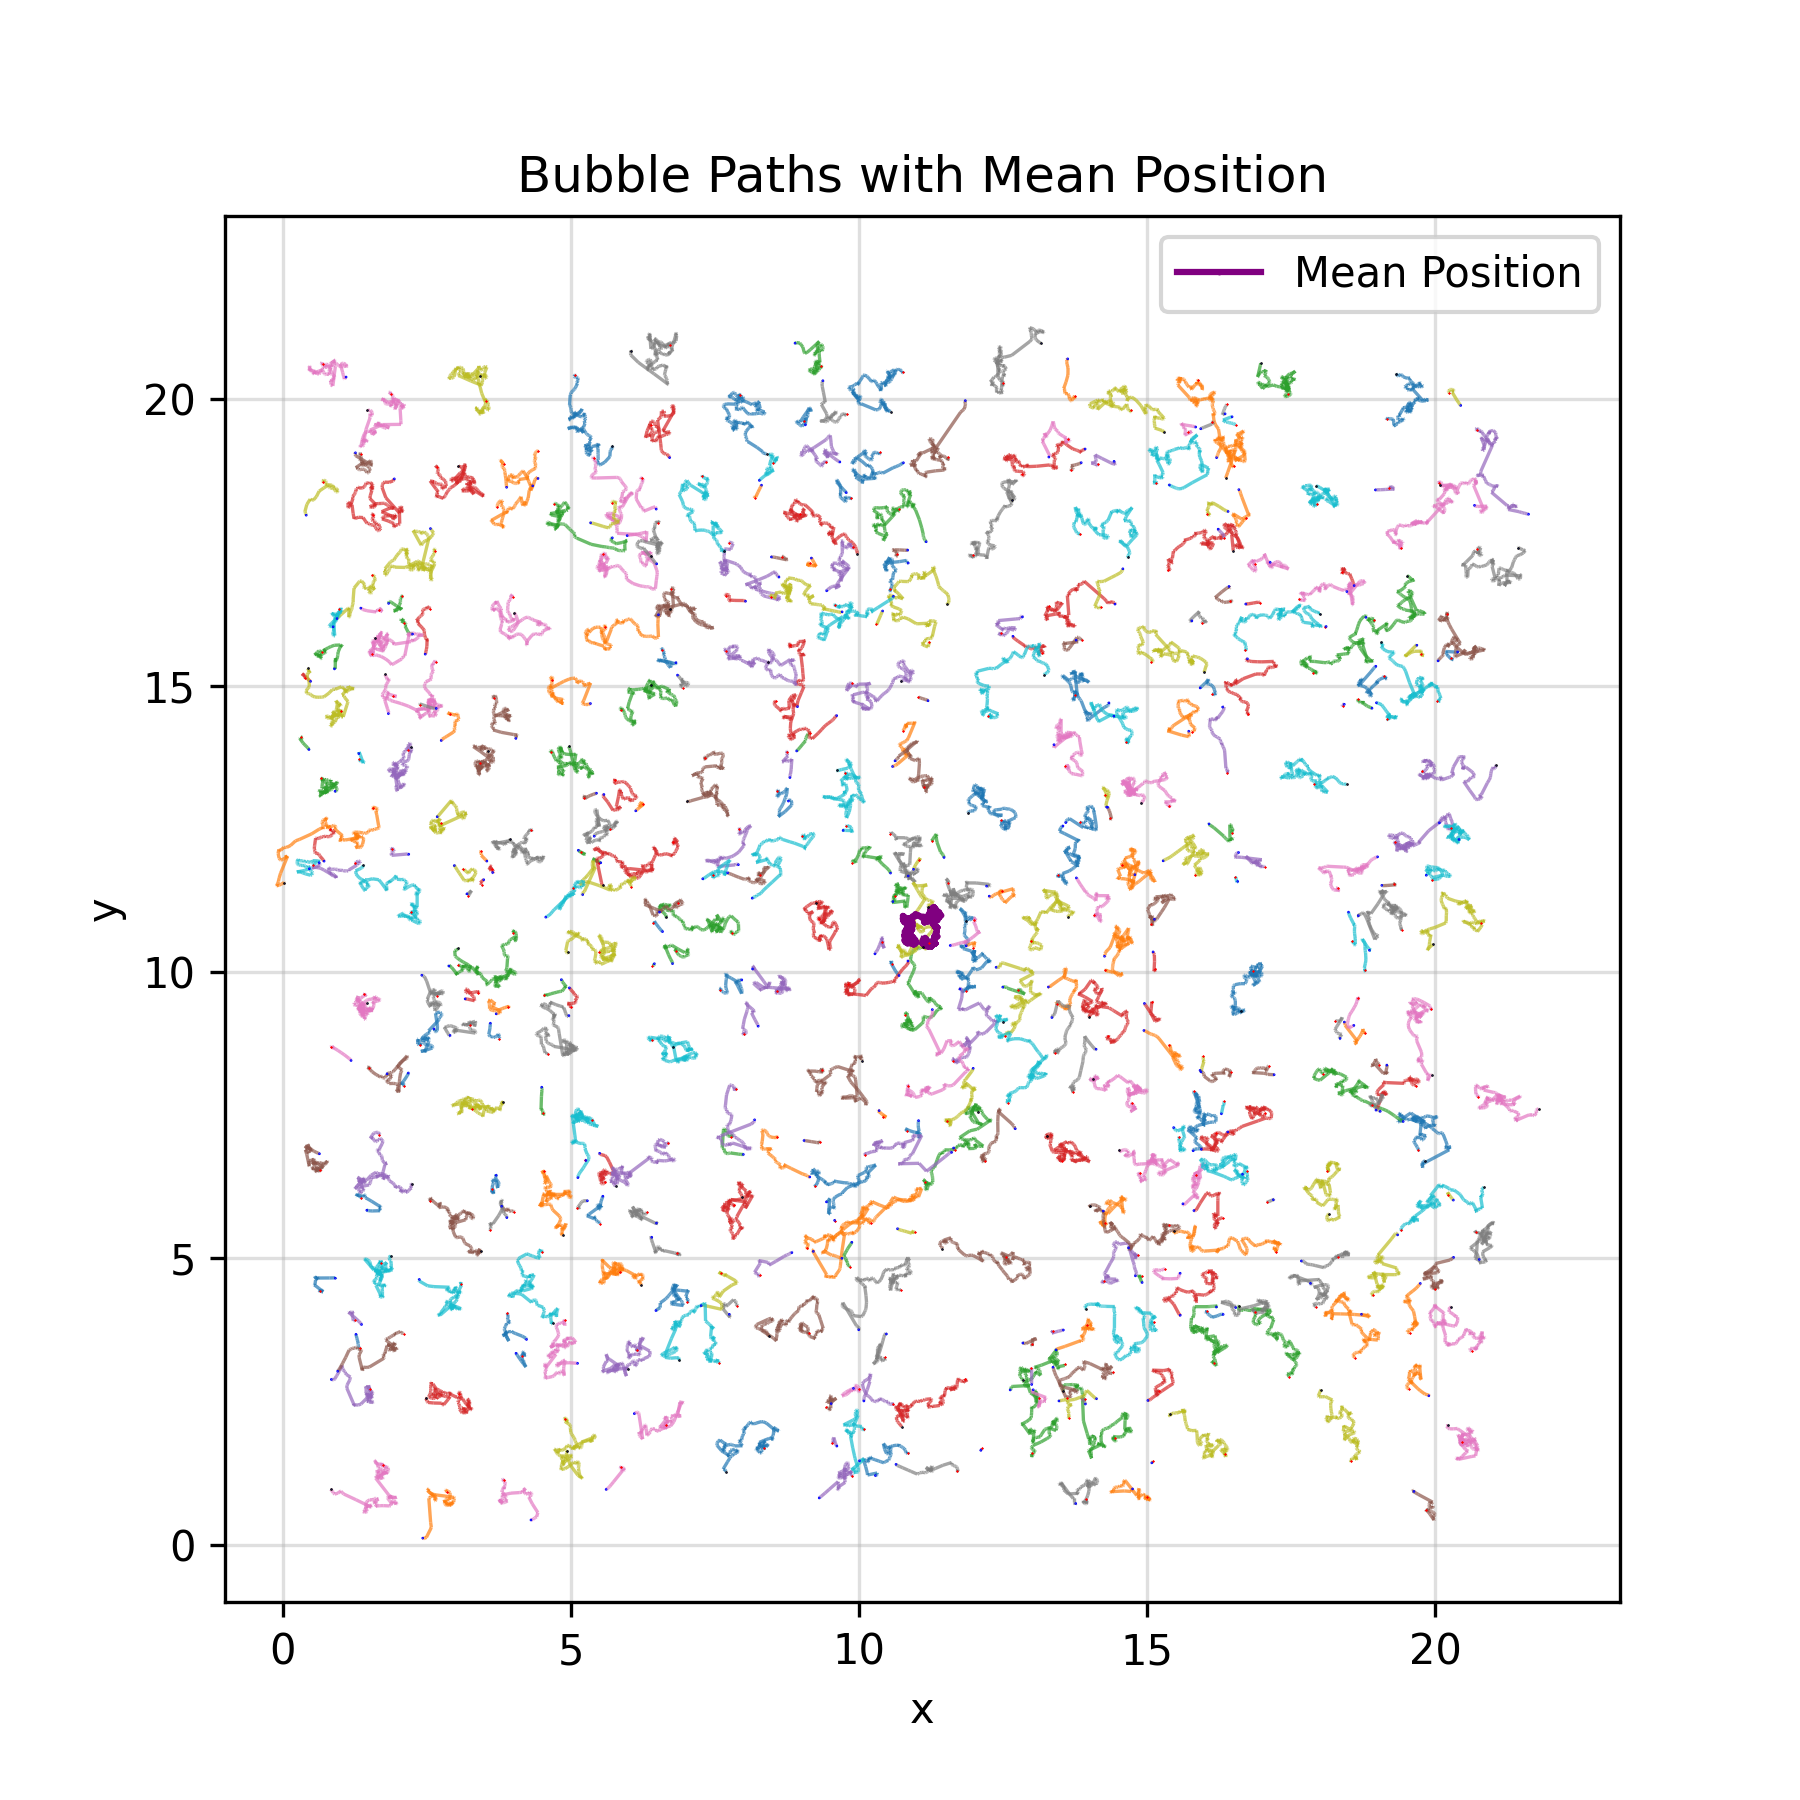
\includegraphics[width=0.45\textwidth]{figures/bubblepathwithmean.png}
    \caption{Paths of the centres of the bubbles.}
    \label{bubbleallpath}
\end{figure}
Figure \ref{bubbleallpath} shows the path of the centres of the bubbles during the simulation. The mean position of the bubbles is shown in the centre of the plot to investigate for an overall drift in the bubbles. Mainly, this is to prove that there is no bias in displacements in the x and y direction, so when we look at the distribution of displacements, we can combine the x and y displacements for double the data.\\
\newpage

\begin{figure}[h!]
    \centering
    \begin{minipage}[t]{0.49\textwidth}
        \centering
        
\includegraphics[width=\textwidth]{figures/Gaussian_rand_walk.png}
        \label{zoombrown}
    \end{minipage}
    \hfill
    \begin{minipage}[t]{0.49\textwidth}
        \centering
        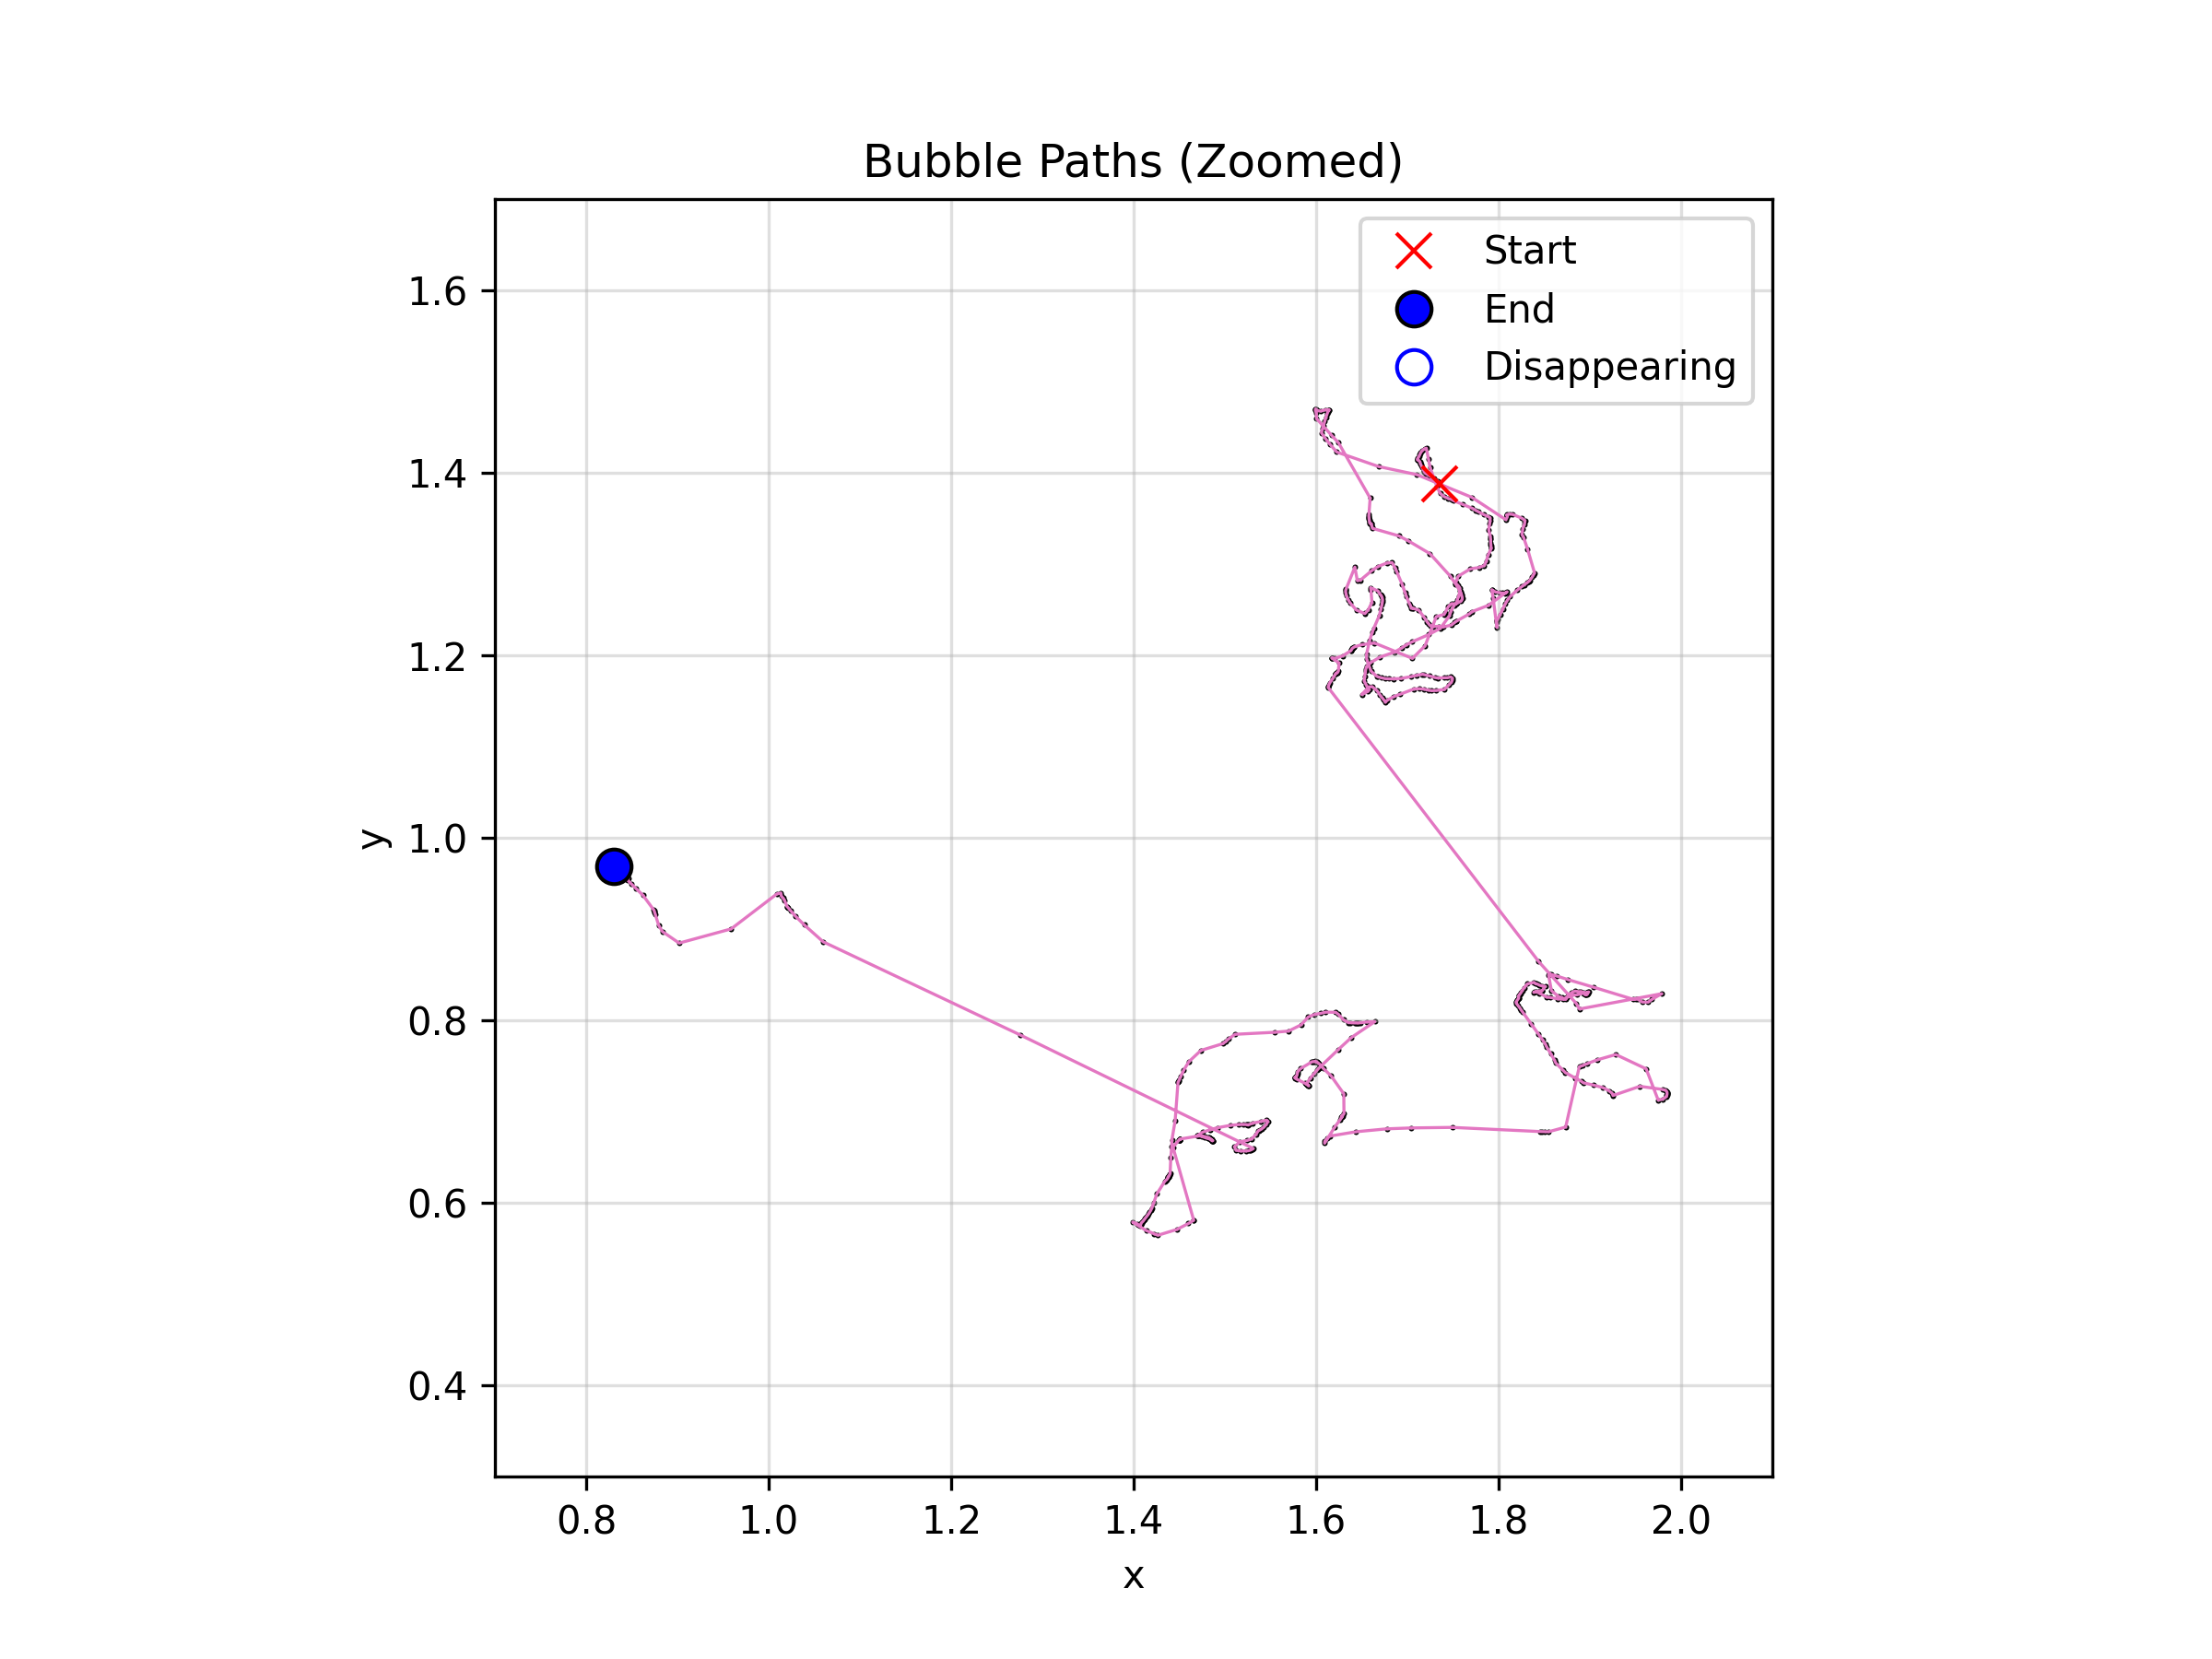
\includegraphics[width=\textwidth]{figures/BubbleWalkZoom.png}
        \label{zoombubble}
    \end{minipage}
    \caption{Comparison of a Brownian random walk (left) and a tracked bubble path (right) over the same number of timesteps.}
    \label{fig:walk_comparison}
\end{figure}
Figure \ref{fig:walk_comparison}a shows a Brownian random walk over 726 steps, the same number of time steps in the foam simulation. Figure \ref{fig:walk_comparison}b shows the path of one of the bubbles which survives the full 726 timesteps. Comparing the two side by side, it is clear that the Brownian random walk is completely random, erratic, and uncorrelated. Whereas the bubble path seems slightly more structured, with some steps clustered together, when the foam is relaxed, and some large jumps then the foam is restructuring. This is a stark difference between the two, however it is worth comparing with the Brownian walk as a baseline to see how random, or what particular type of randomness, the bubble paths follow.\\


% \begin{figure}[h]
%     \centering
%     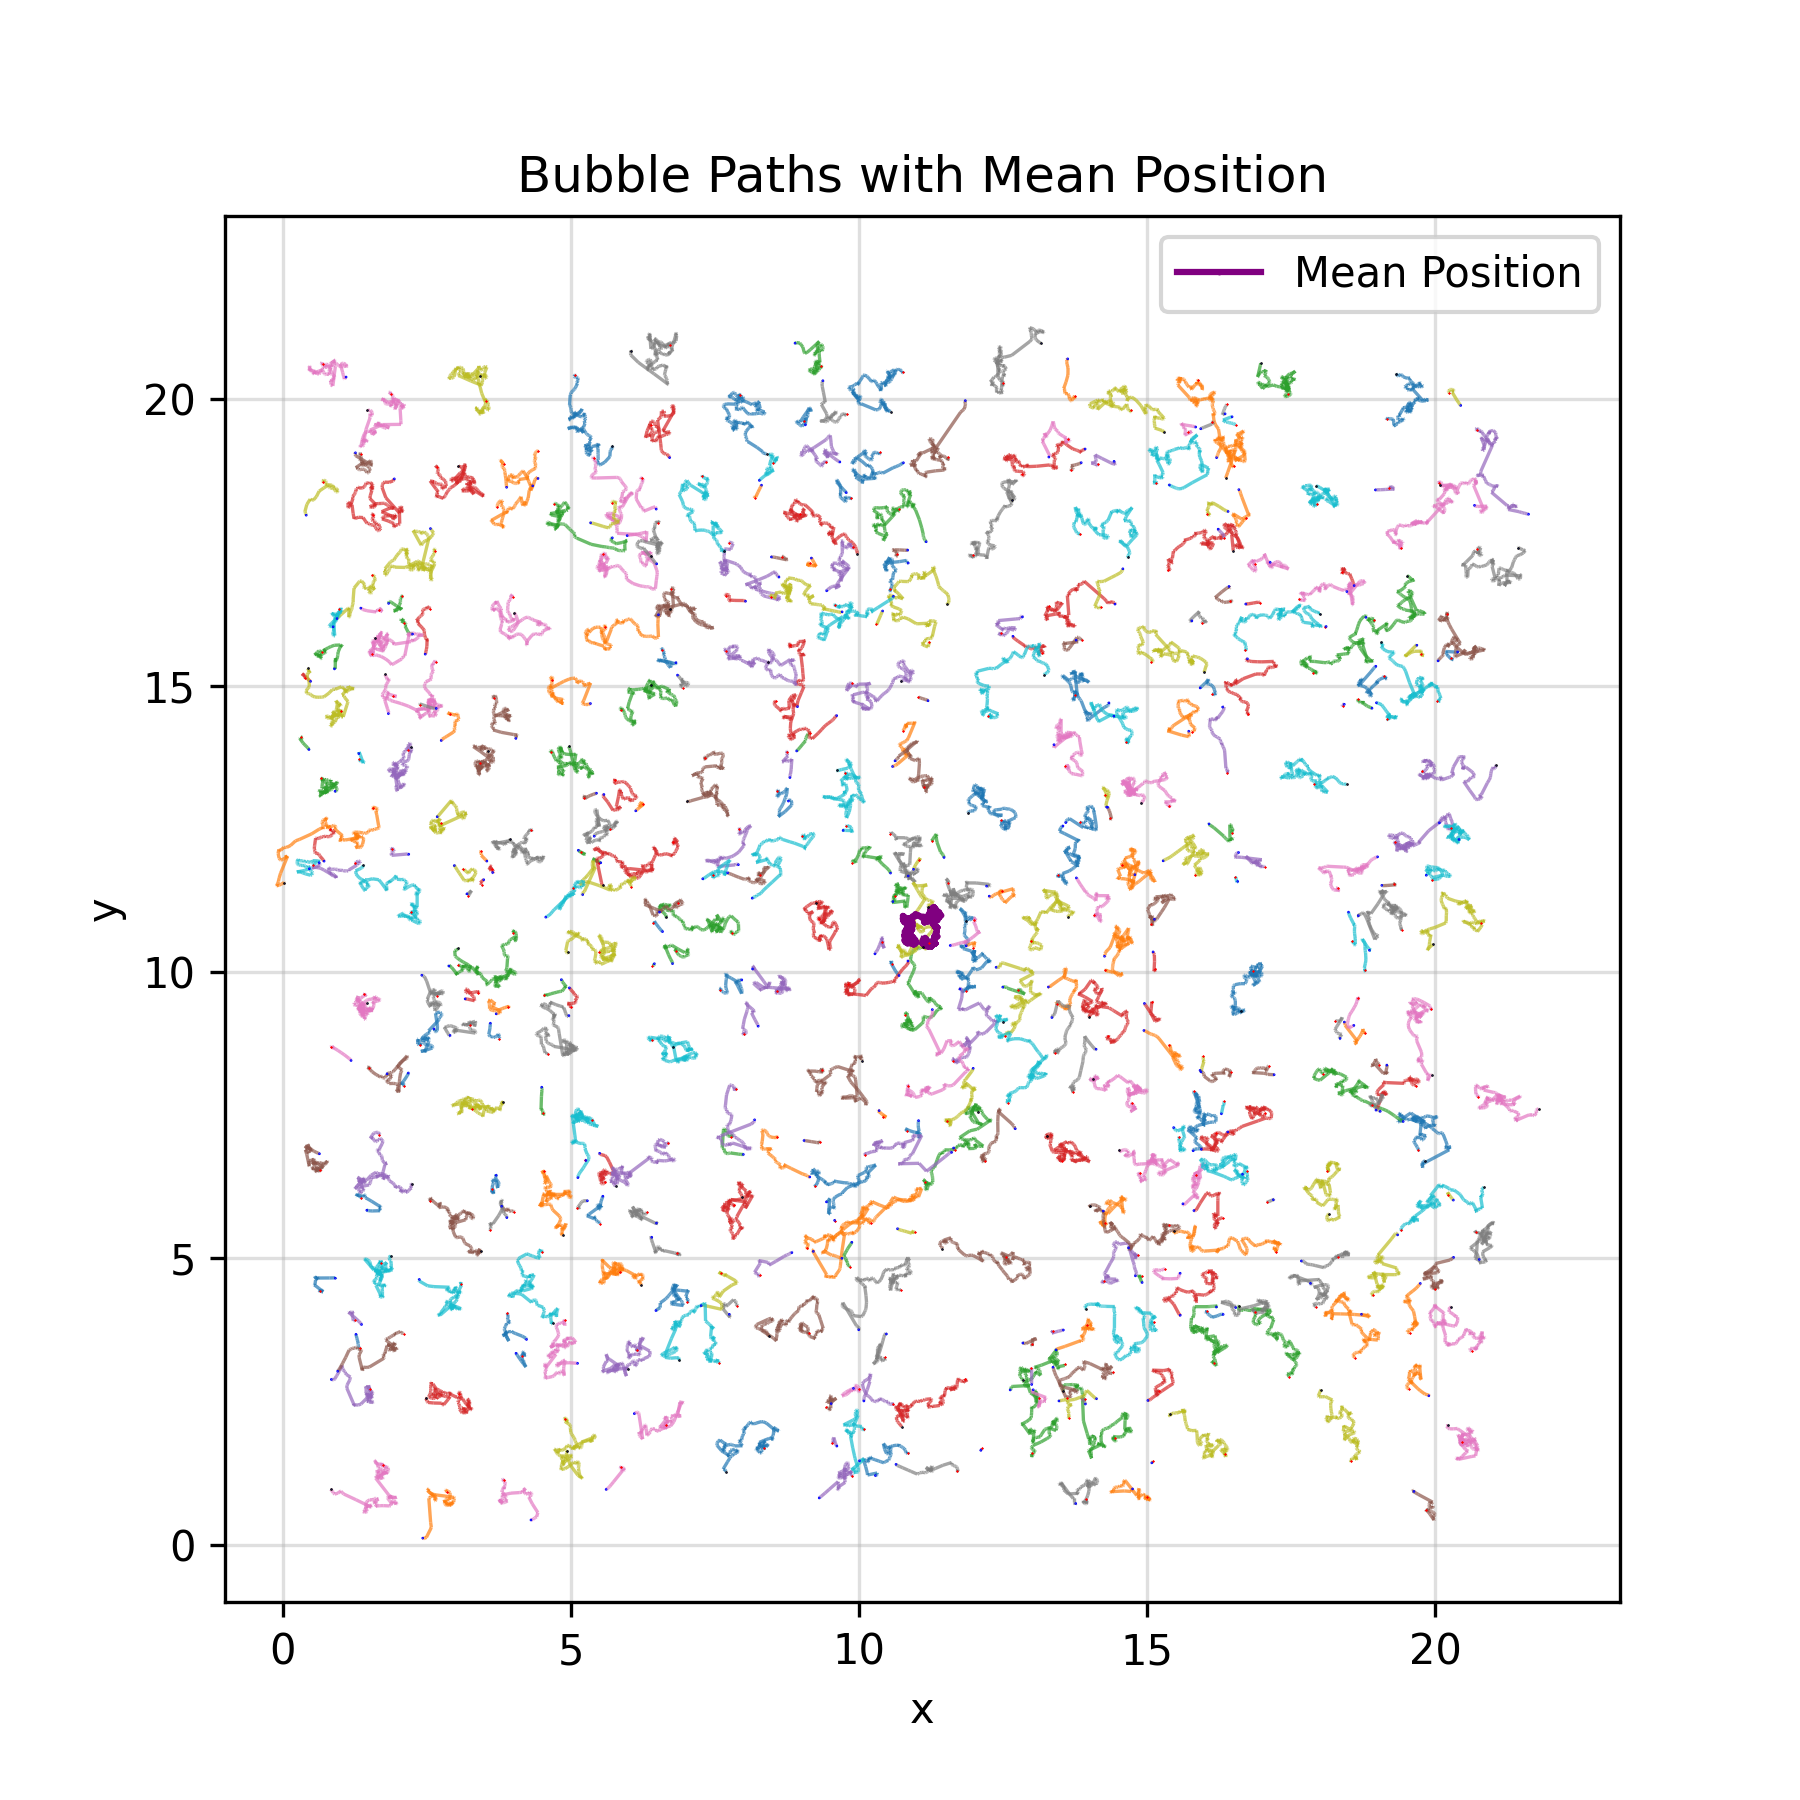
\includegraphics[width=\textwidth]{figures/bubblepathwithmean.png}
%     \caption{The centres of the bubbles tracked over the full simulation, some disappearing before the simulation is finished, some survive till the end. \textcolor{red}{put in appendix maybe}}
% \end{figure}

% \begin{figure}[h]
%     \centering
%     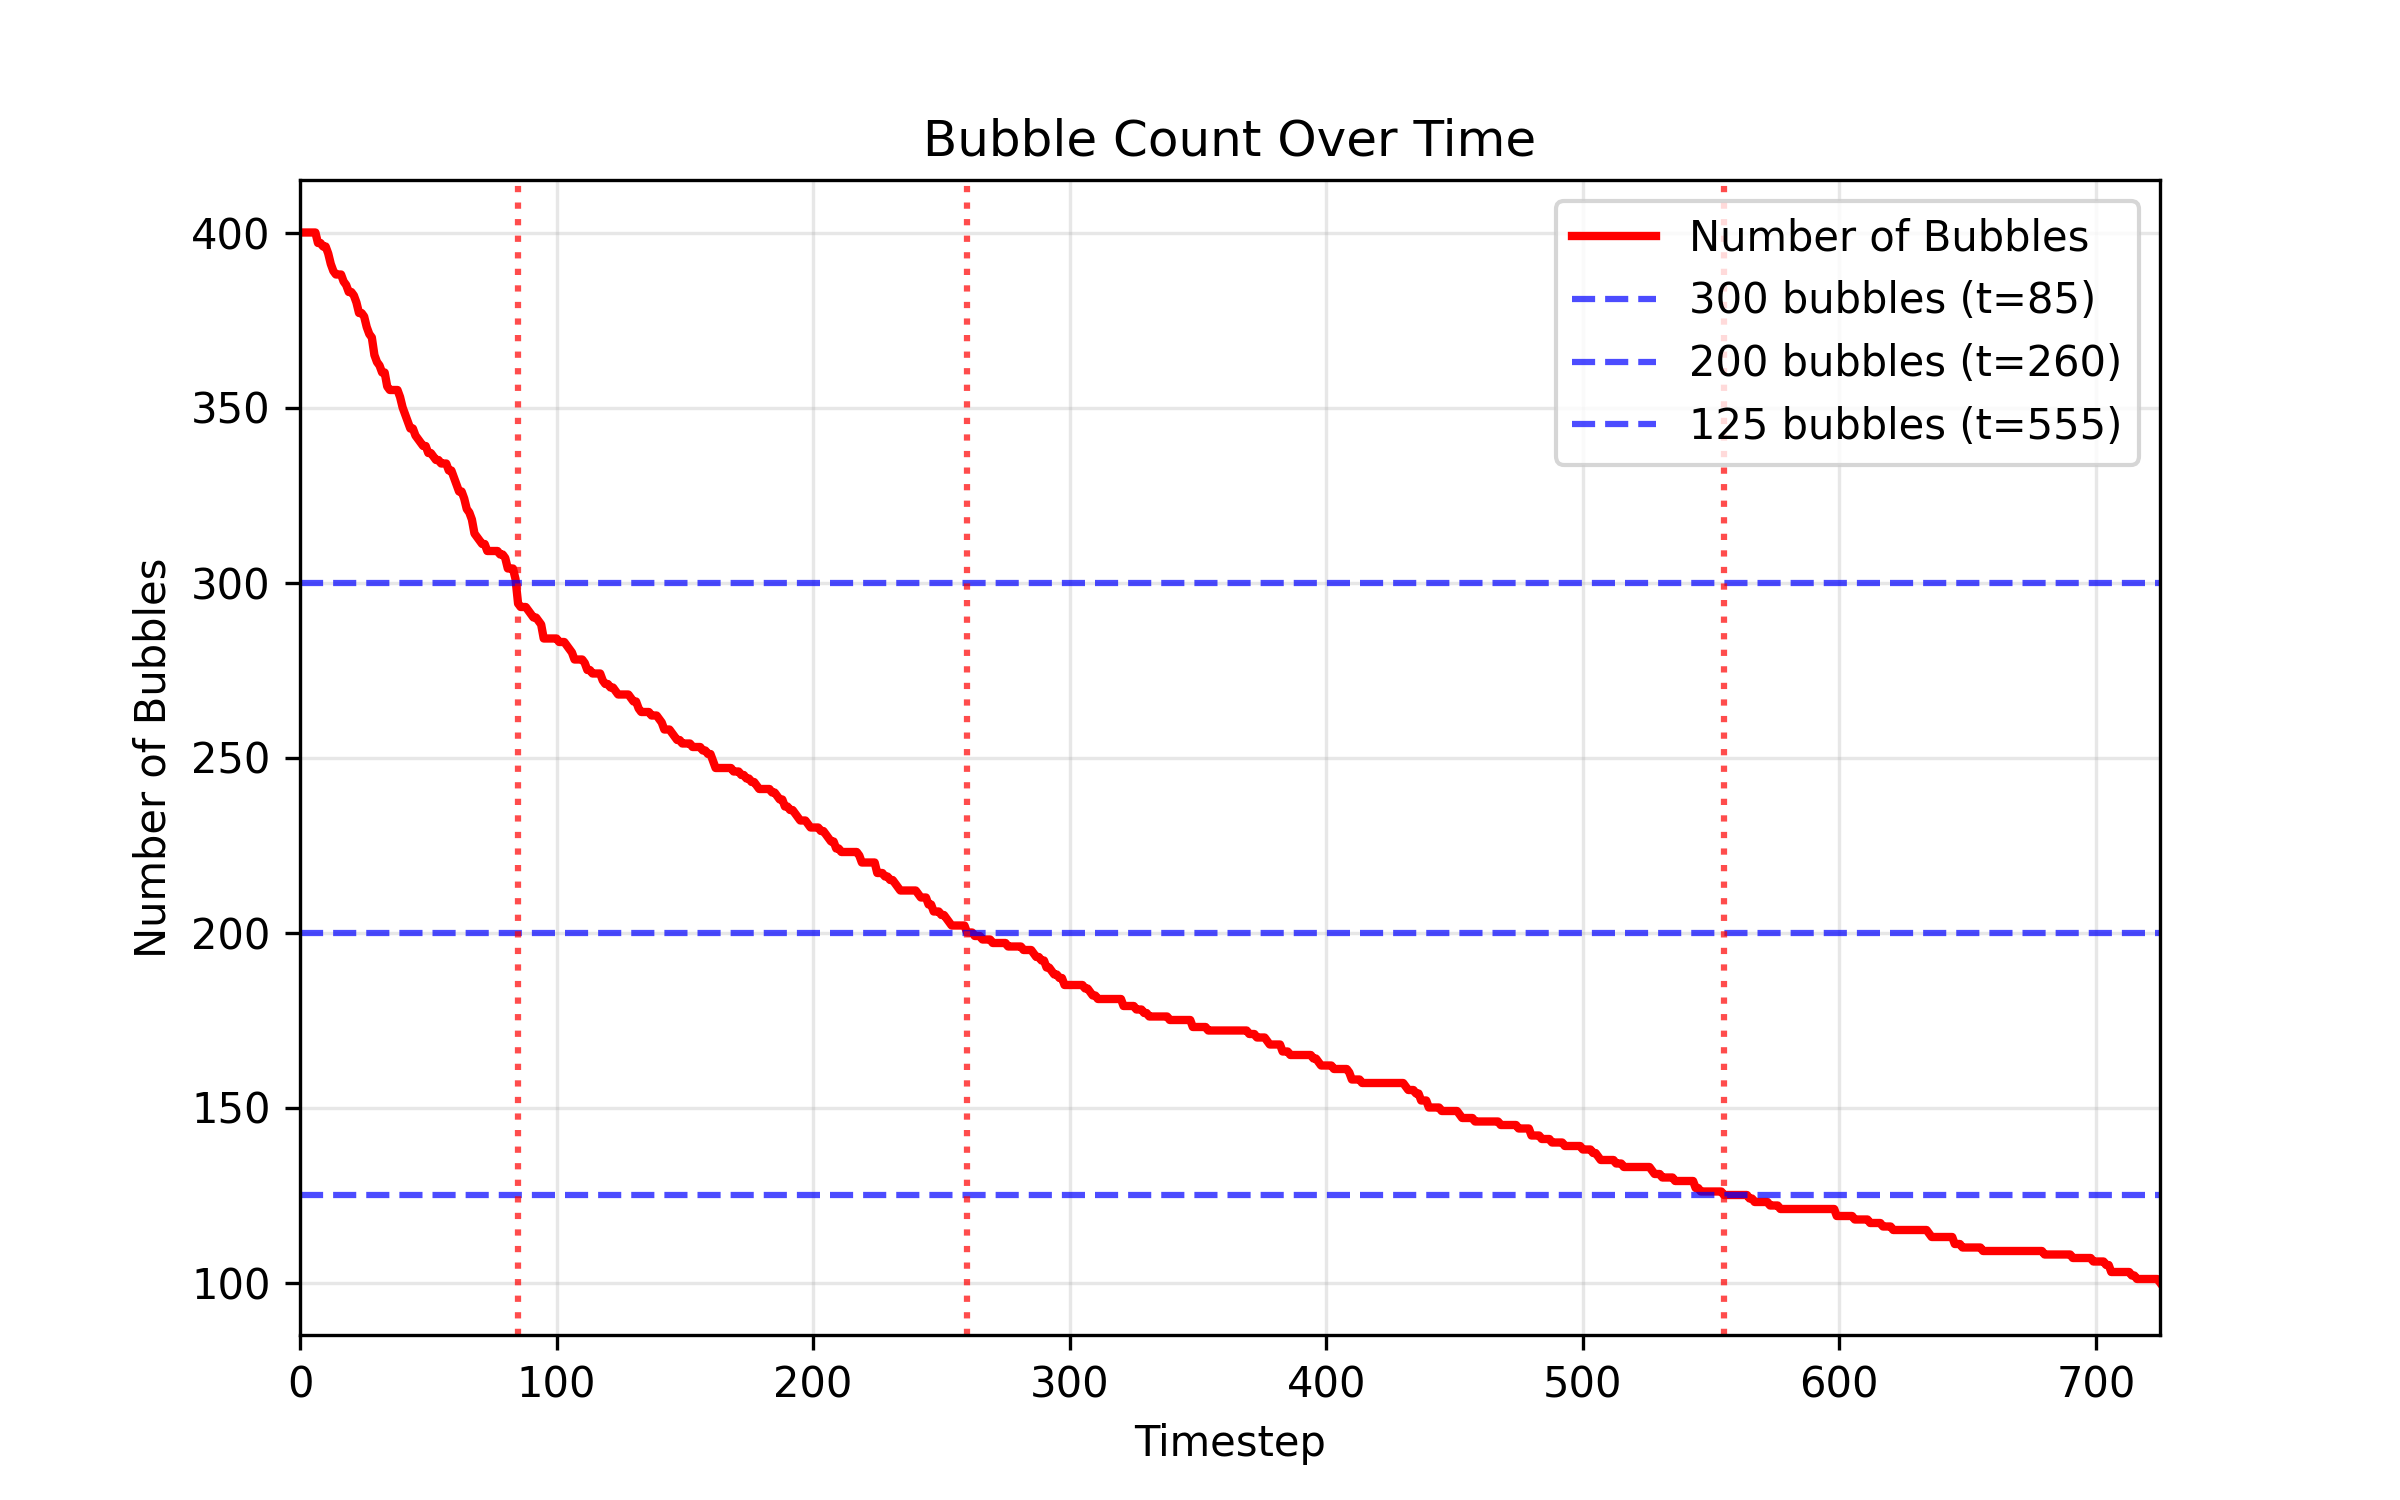
\includegraphics[width=\textwidth]{figures/bubble(MSD)_count_over_time.png}
%     \caption{\textcolor{red}{put in appendix}}
%     \label{survival_curve}
% \end{figure}

\subsubsection{Average Area}
As a sanity check, the average area over time is shown to be linear in figure \ref{fig:areaavg}. This was proven in two ways. The first was using the raw diameter data and averaging that the area obtained from that over all the bubbles in that timestep, The second method used an approximation, $\langle A \rangle = A_{box}(1-\phi)/N(t)$, where $\phi$ is the liquid fraction and $N(t)$ is the number of bubbles at time t. Figure \ref{fig:areaavg} proves these two methods line up exactly.\\

The key takeaway from this is that since the area is increasing linearly with time then we are losing bubbles while this is happening.

\begin{figure}[h!]
    \centering
    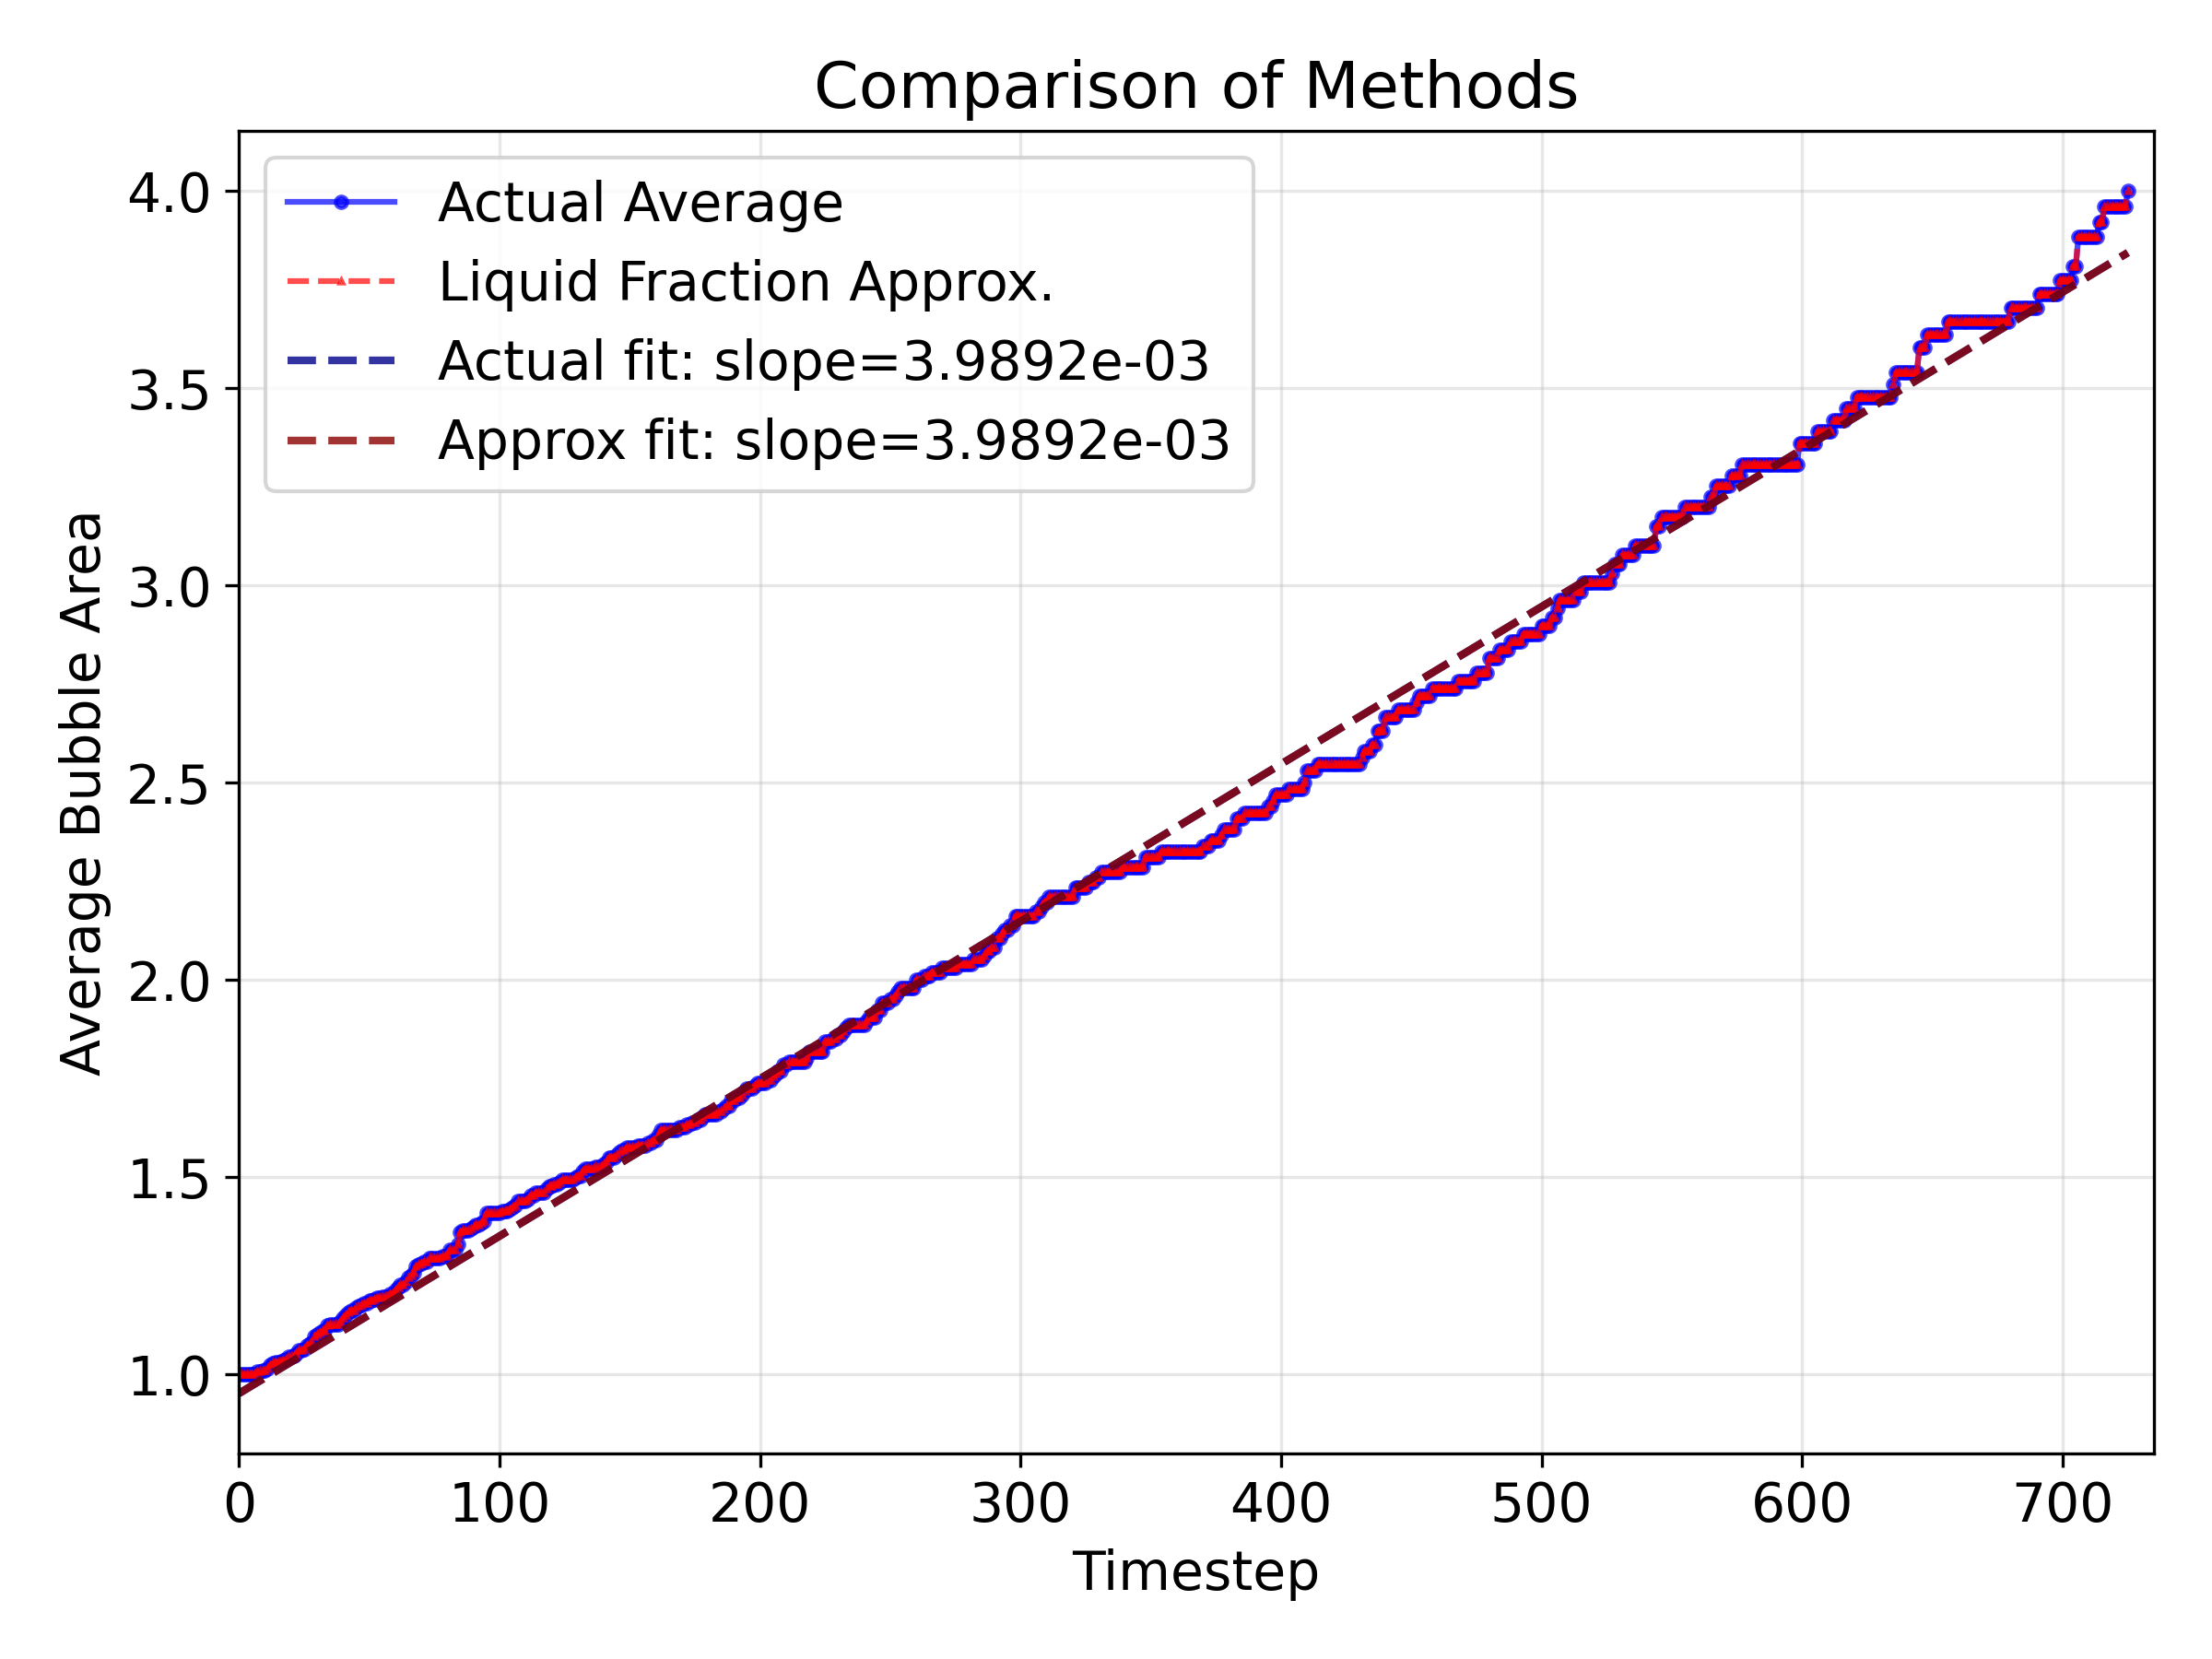
\includegraphics[width=0.5\textwidth]{figures/comparison_bubble_area_methods.png}
    \caption{Average bubble area increases linearly over time.}
    \label{fig:areaavg}
\end{figure}

\subsubsection{Mean Squared Displacement}
\begin{figure}[H]
    \centering
    \begin{minipage}[H]{0.45\textwidth}
        The mean squared displacement (MSD) was averaged over 400 Brownian random walks, and as expected scaled linearly with time. In figure \ref{fig: MSD}, this Brownian MSD line is superimposed onto the plot of the bubbles MSD over time. There are some stark differences. Initially, since I was looking for this linear relation in the bubbles I tried to convince myself there was some sort of linearity in the plot. While there certainly is an upward trend, it is definitely not linear, at least not with the amount of data we have.
    \end{minipage}
    \hfill
    \begin{minipage}[H]{0.53\textwidth}
        \centering
        
\includegraphics[width=\textwidth]{figures/bubble_MSD_alongside_Gaussian400.png}
        \caption{Hard to draw conclusion from bubble MSD}
        \label{fig: MSD}
    \end{minipage}
\end{figure}

One clear distinction between the two simulations is that the number of bubbles decrease over time. This can be seen in the figure \ref{fig: MSD} with the red dashed lines marking the milestones in the bubble counts. As the number of bubbles decrease, the statisics are average over fewer paths, leading to increased noise making it harder to determine a linear relation. An example of this is plotting the Brownian MSD averaged over 100 walks imposed on a plot of MSD averaged over 400 walks(Appendix B: Figure \ref{fig:100vs400}). Averaging over a smaller number of trajectories leads to a noticable increase in noise. When analysing the bubble MSD, this can be seen once half the bubbles have disappeared around the 260th timestep. Having said that, even when we have the most amount of bubbles, 400-300 bubbles between t=0 and t=80, this section of the plot almost looks like it follows a power law so it is hard to draw conclusions from this investigation.\\

The conclusion from this investigation is that it is hard to make any good conclusions from this analysis. For that reason, we move on to other method to analyse the statistics of this system.


\subsubsection{Displacement Distributions} \label{sec: dispdist}
The displacement distribution of the bubble displacements looking at every timestep ($\Delta t = 1$) has a sharp peak around 0 and tapers down each side, as seen in figure \ref{dispdist} on a log-lin scale. Comparing with the Brownian displacement curve in figure \ref{Browndispdist}, there is a stark difference between the two distributions; an inverted parabola for the Brownian motion, and a sharp peak for the bubble displacements.\\

\begin{figure}[h]
    \centering
    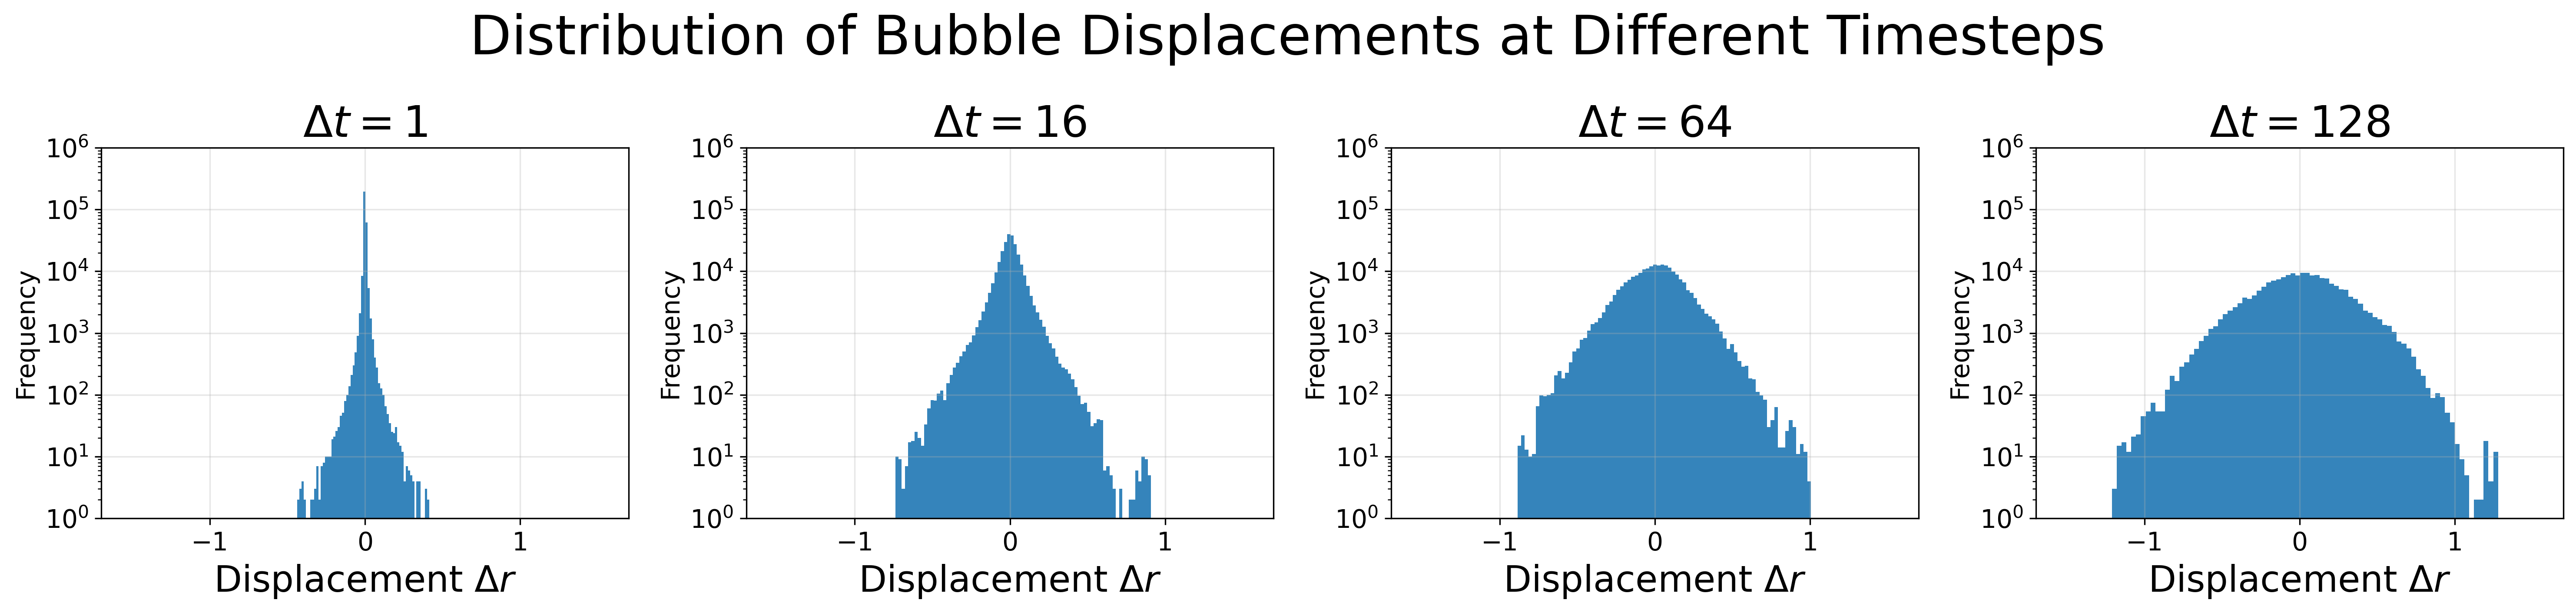
\includegraphics[width=\textwidth]{figures/displacement_distributions_1x4.png}
    \caption{Displacement distributions looking at different time lags. Distibutions widen towards a Gaussian distribution at larger time lags.}
    \label{dispdist}
\end{figure}

As $\Delta t$ increases the bubble displacement distributions widen, eventually approaching a Gaussian shaped inverted parabola. This shows the uncorrelation comparing displacement at a certain timestep versus displacement a hundred or so timesteps later. There is an element of randomness which brings the Gaussian distribution into play.\\

\begin{figure}[H]
    \centering
    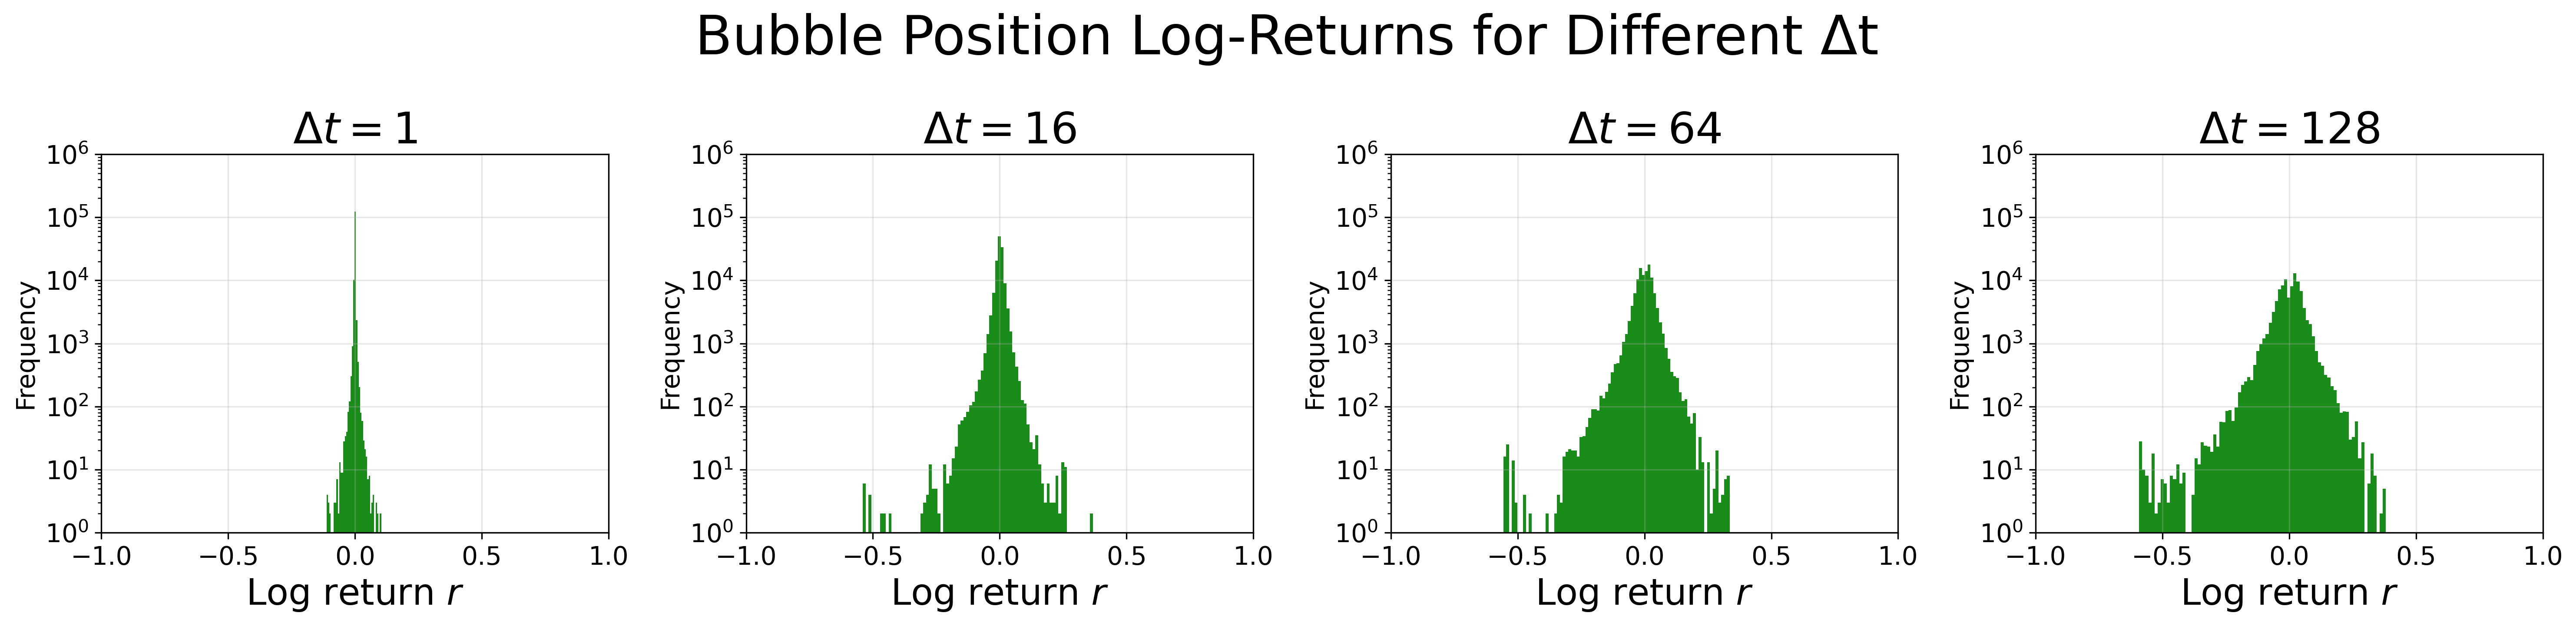
\includegraphics[width=\textwidth]{figures/log_returns_seperate_bubbles_2.png}
    \caption{Log return distributions over increasing $\Delta t$. Distribution does not widen into a Gaussian unlike the displacement distributions. Log-linear scale.}
    \label{logretdist}
\end{figure}

Investigating the log return distributions led to a different conclusion than the displacement distributions. Unlike the displacement distributions, the log return distribution does not widen into a Gaussian curve. As the distribution don't evolve into a Gaussian, section \ref{subsec: Autocorrelation} will investigate if there is an element of time correlation in the log returns.\\


\subsubsection{Complementary Cumulative Distribution Functions Collapse}
As confirmation of the CCDF collapse method used in this project, the Brownian walk distributions (both displacement and log returns) collapse as intended onto one master curve, \textit{see Appendix B: Figures \ref{fig:BrownCCDF1} - \ref{fig:BrownCCDF4}}. One observation in particular is that the CCDF cuts scale exactly linearly with the time lag $\Delta t$ with a slope of 0.5. This was to be expected as the displacements for the Brownian walk are chosen from a Gaussian distribution with standard deviation which scales as $\sigma(\Delta t) \sim \sqrt{\Delta t}$ \cite{PINSKY2011391}. Since the entire distribution rescales with $\sigma(\Delta t)$, every quantile, including $X(C, \Delta t)$ must scale the same way. $X(C, \Delta t) \sim \sigma(\Delta t) \sim \Delta t^{0.5}$.\\

Displacement distributions from the section \ref{sec: dispdist} were used for an initial attempt at a Complementary Cumulative Distribution Function (CCDF) collapse.

\begin{figure}[H]
    \centering
    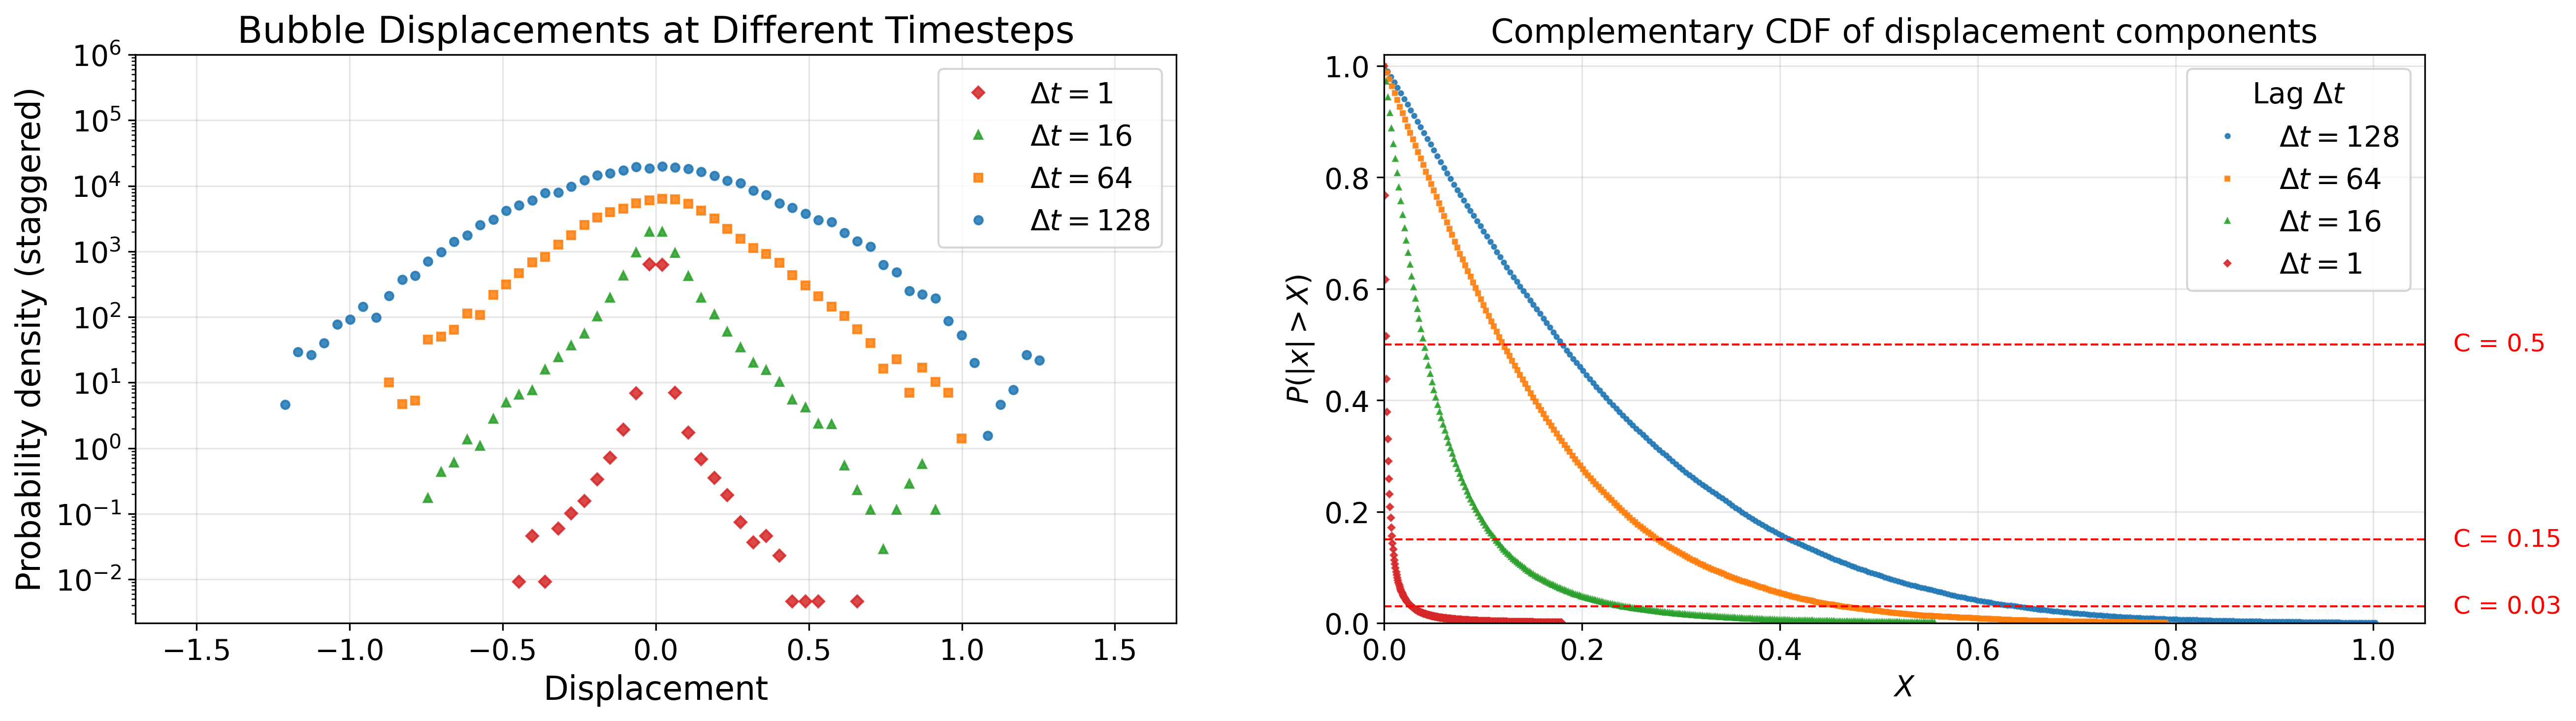
\includegraphics[width=\textwidth]{figures/ccdf_displacement_components_1x2.png}
    \caption{Displacement distributions overlayed on the one plot, axes shifted for visual purposes (left). These PDFs were then integrated over $|x|>x$ to get the CCDF (right).}
    \label{label}
\end{figure}


\begin{figure}[H]
    \centering
    \begin{minipage}[t]{0.49\textwidth}
        \centering
        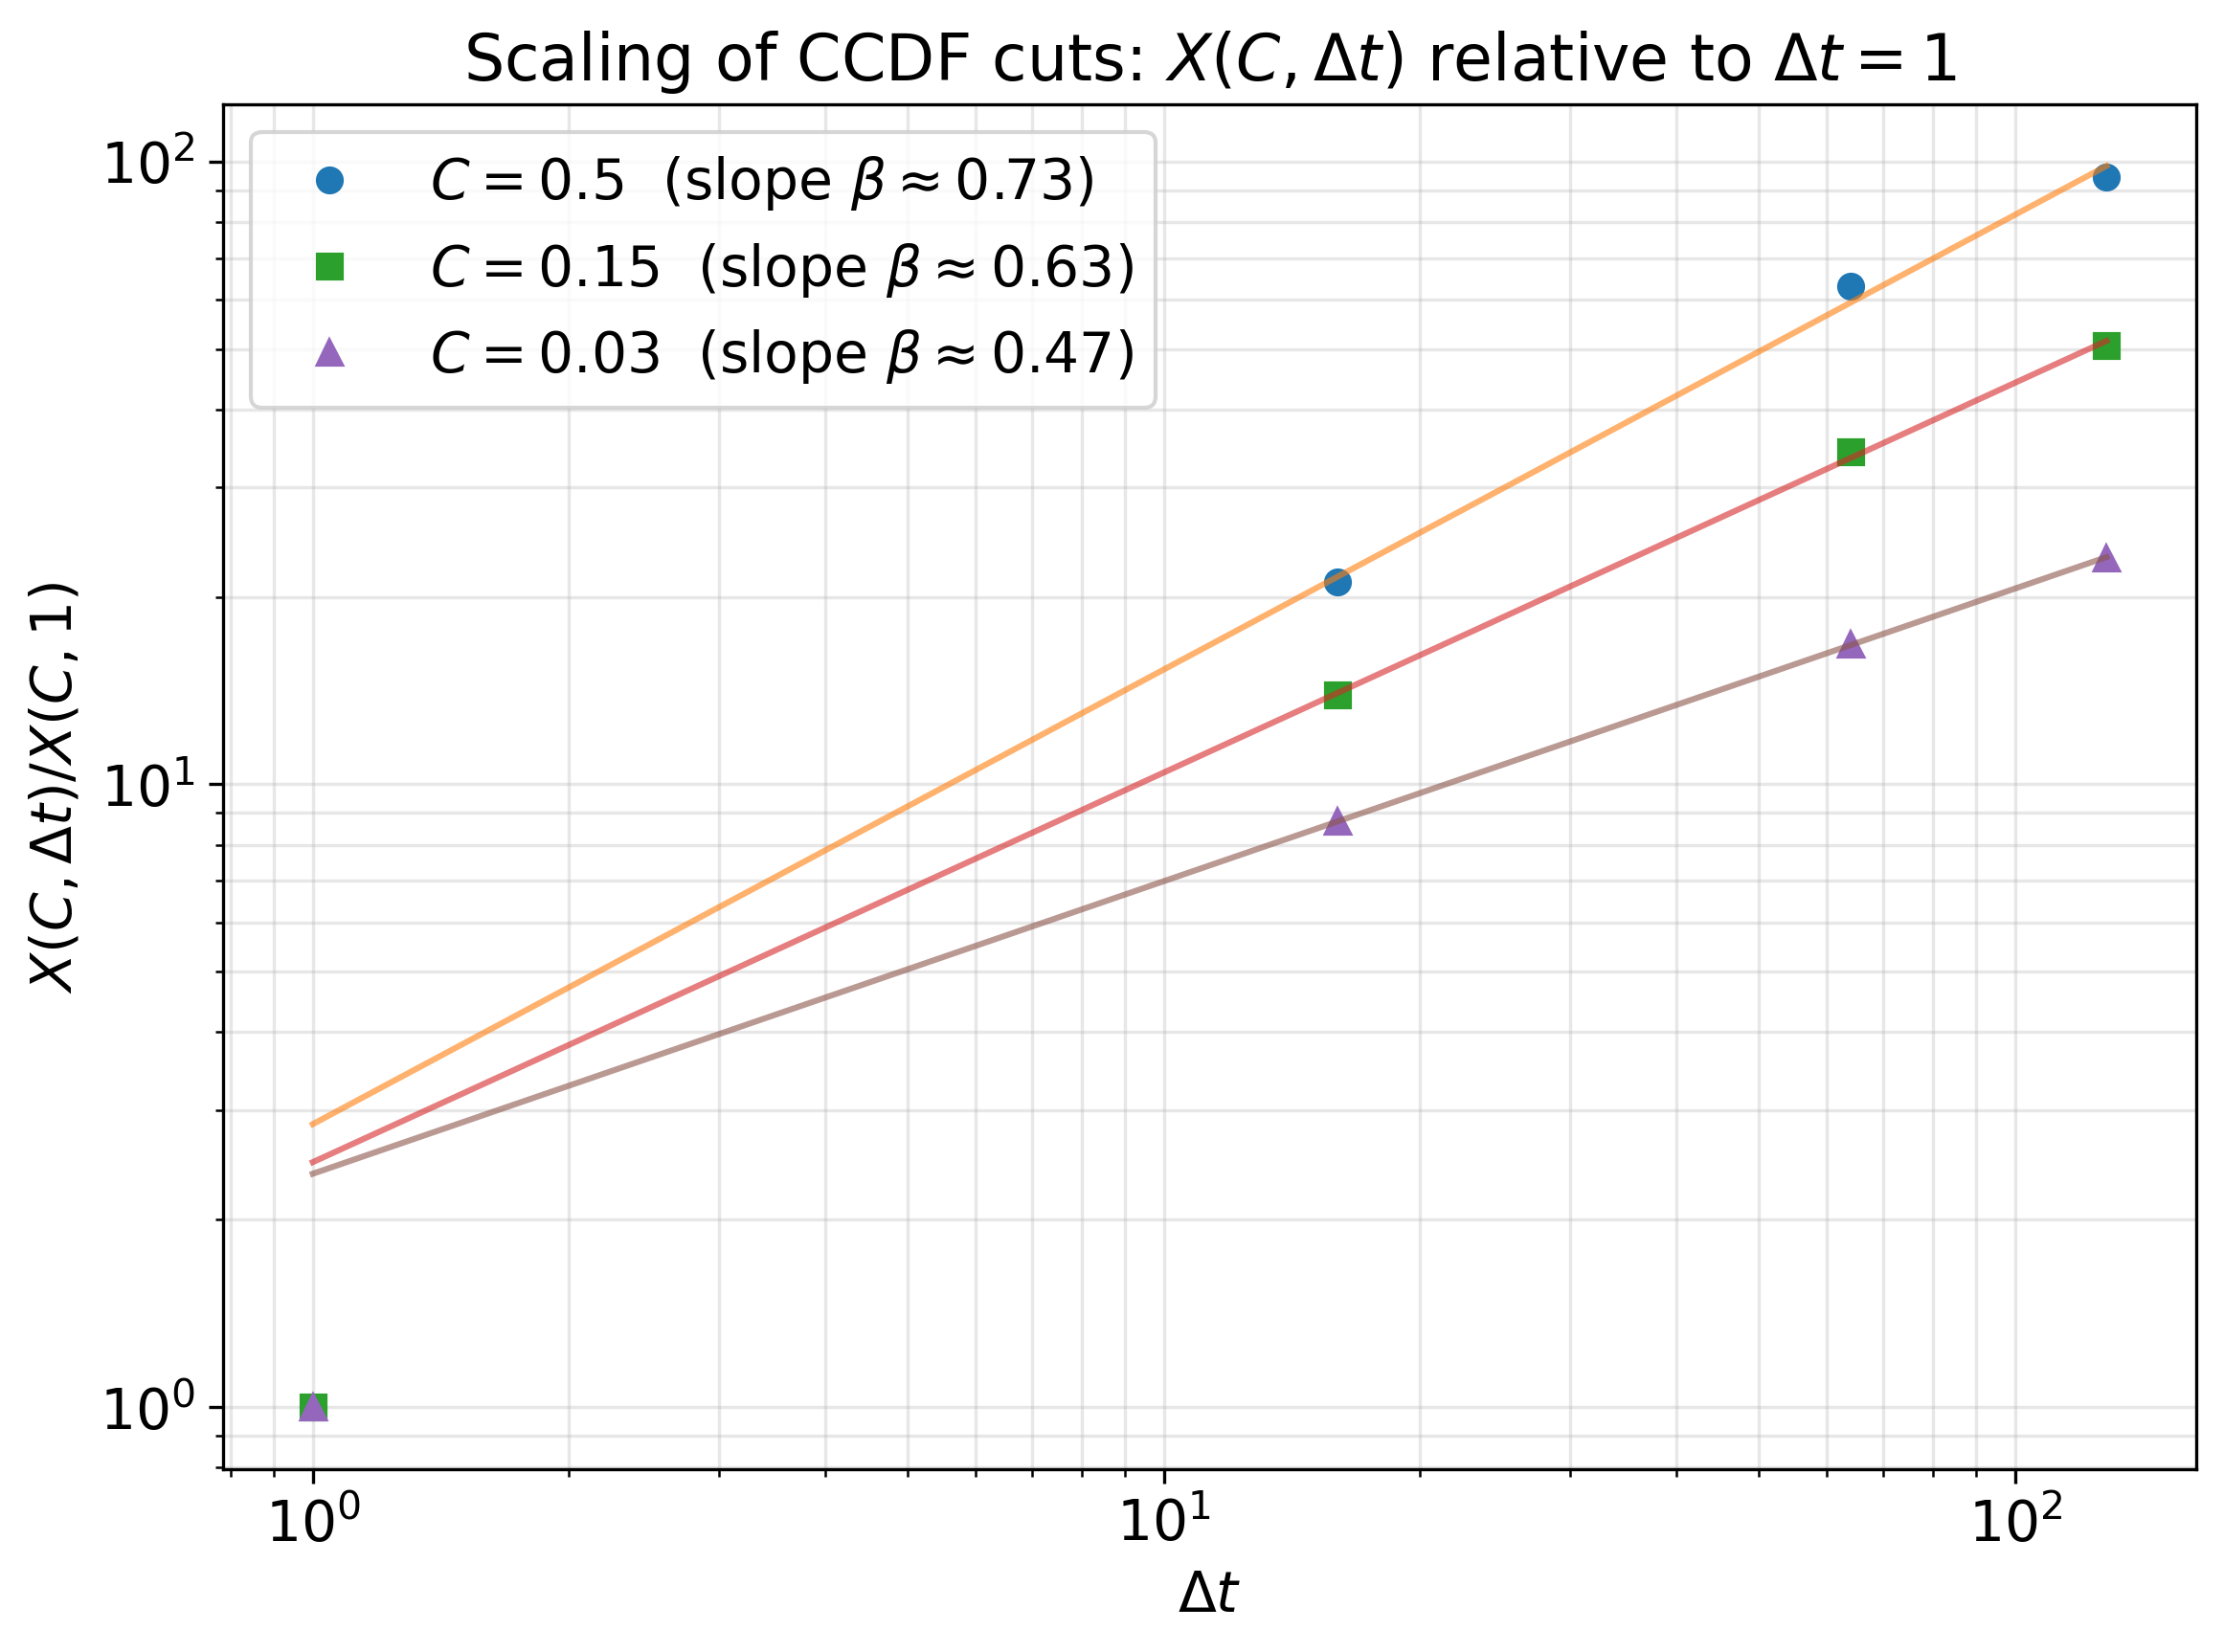
\includegraphics[width=\textwidth]{figures/ccdf_cut_scaling_1.png}
        \label{ccdfcut}
    \end{minipage}
    \hfill
    \begin{minipage}[t]{0.49\textwidth}
        \centering
        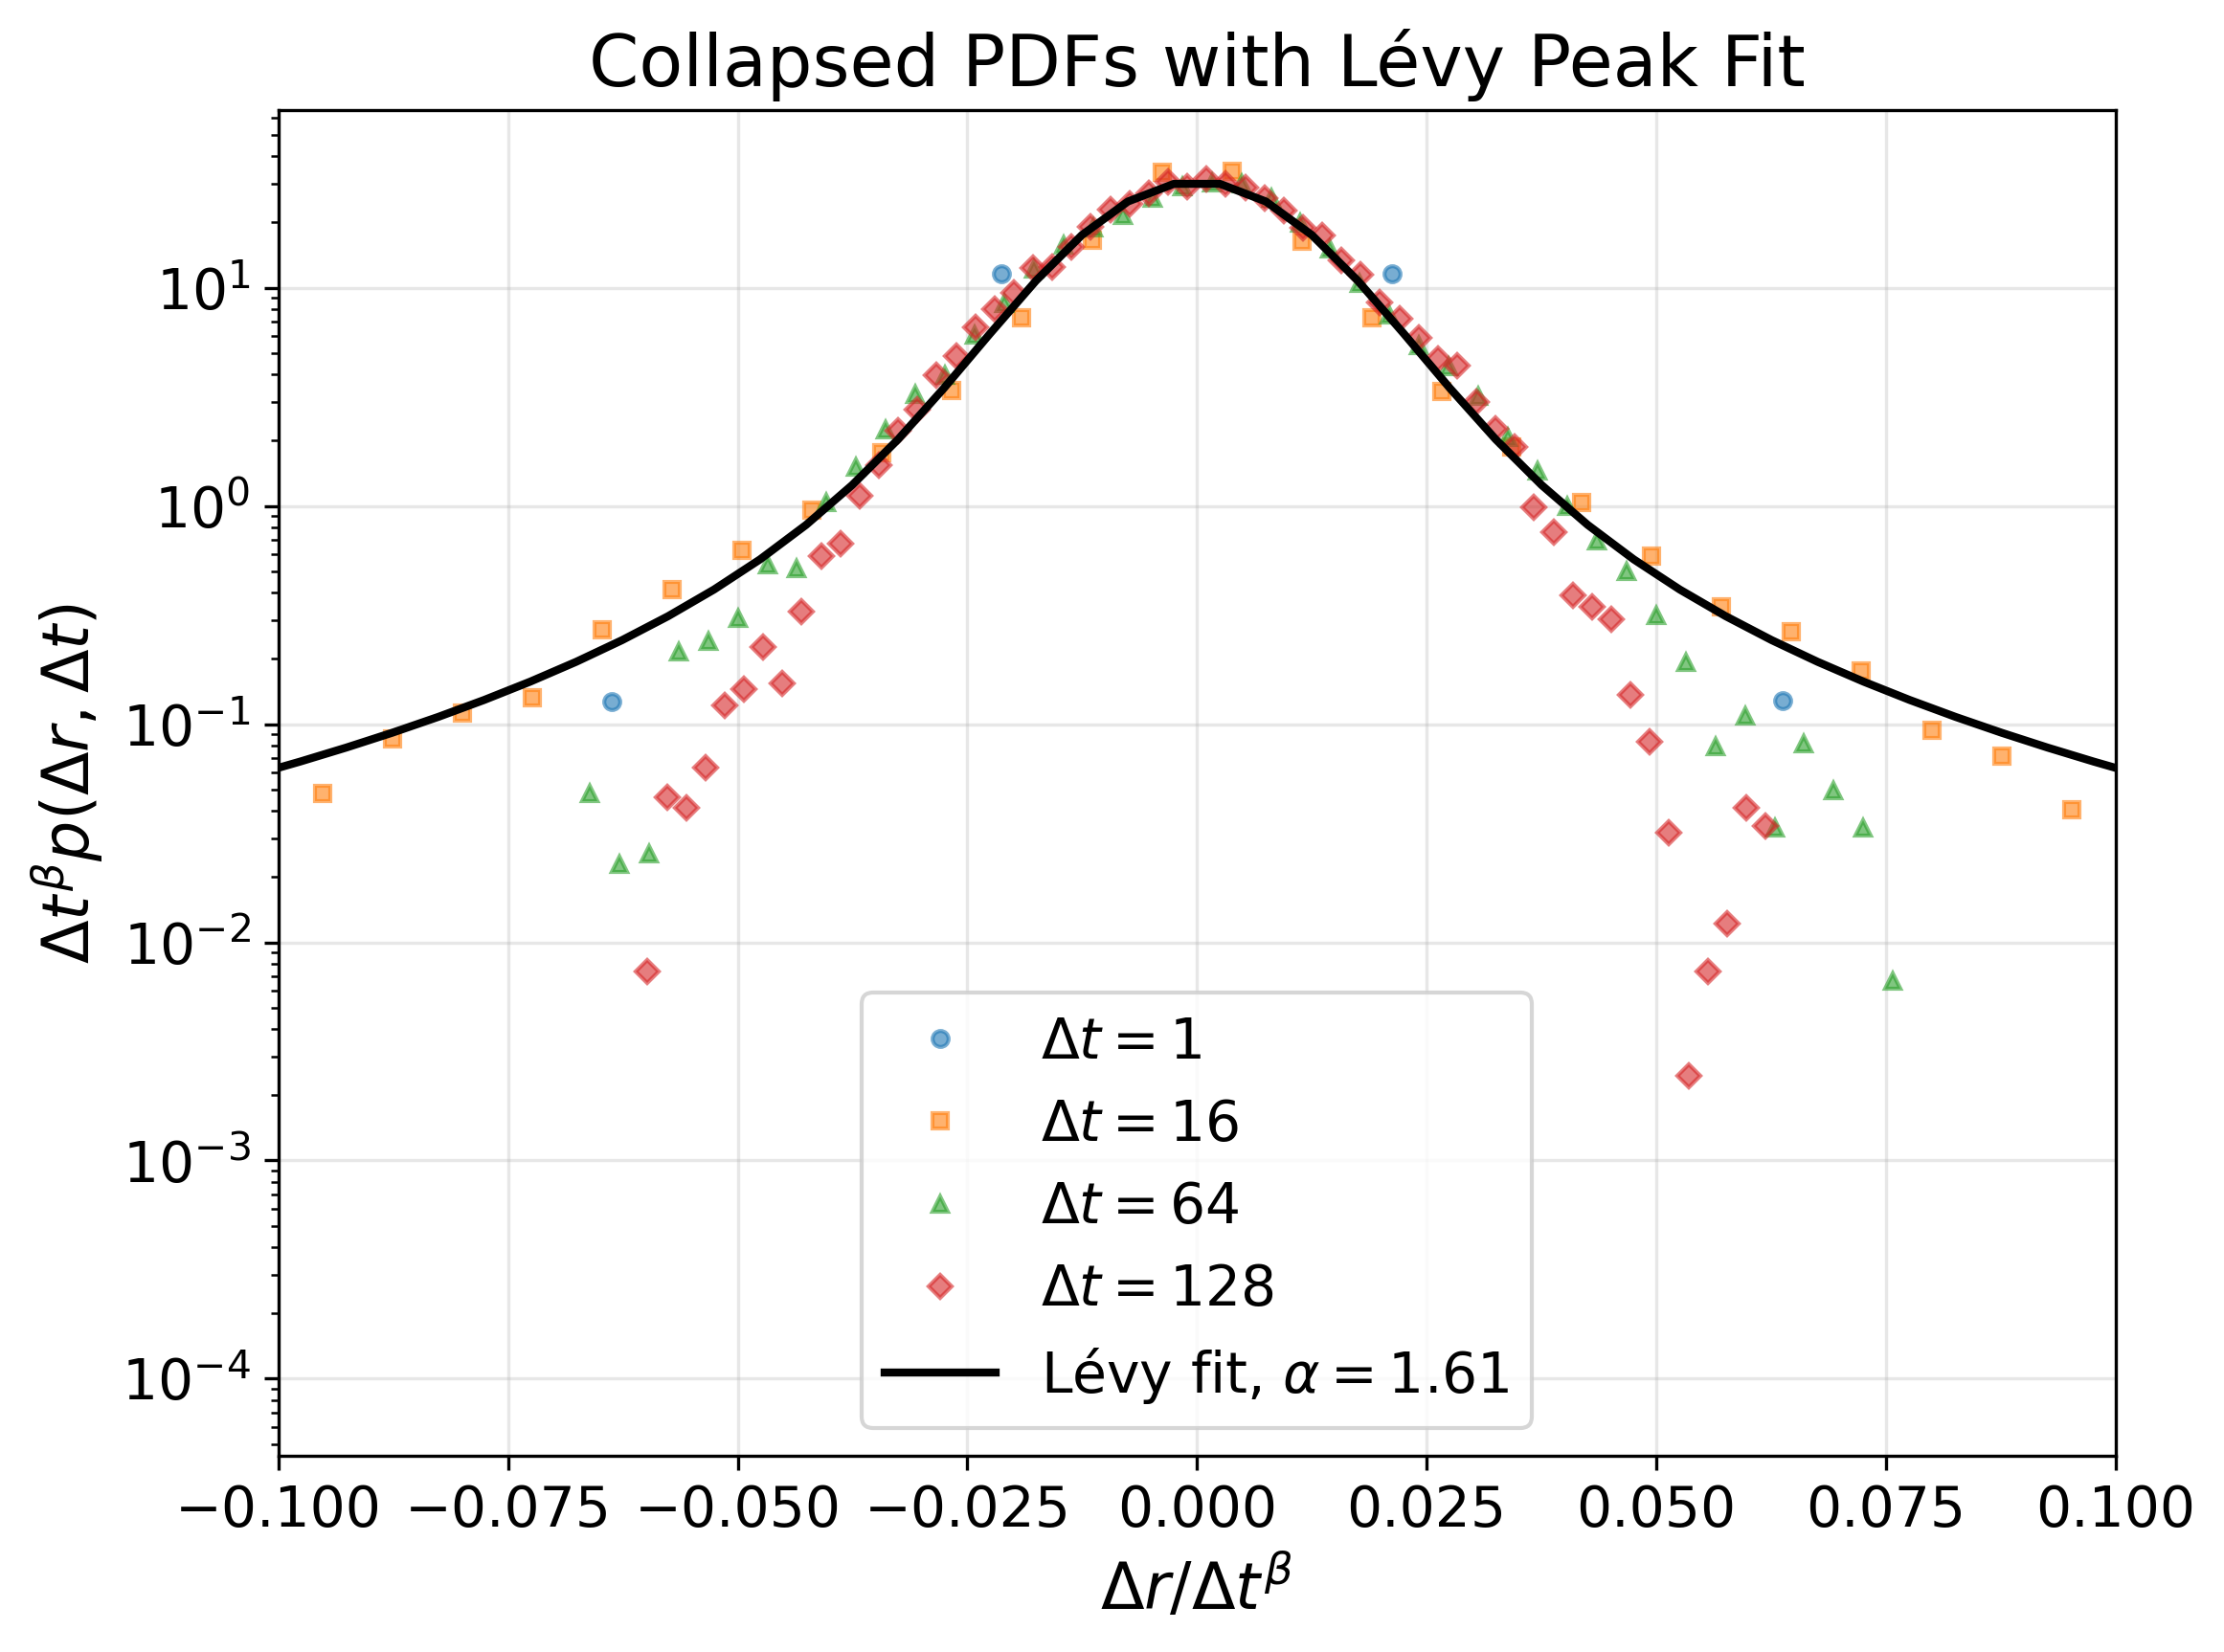
\includegraphics[width=\textwidth]{figures/displacement_pdf_collapse_levy_fit_1.png}
        \label{levycoll}
    \end{minipage}
    \caption{Bubble displacements do not scale according to Levy distribution.}
    \label{fig:cutandcollapse_1}
\end{figure}

A key difference between the bubble displacement distribution scaling and the scaling of financial markets is that the CCDF cuts are dependent on where the cut is taken, there is not a linear relation between the cut (normalised to the first cut) versus $\Delta t$, \textit{see figure \ref{fig:cutandcollapse_1}a}. For arguments sake, the middle slope is taken, $\beta = 0.63$ giving a relatively good collapse in figure \ref{fig:cutandcollapse_1}. The centre of the distribution collapses well, however, the tails clearly deviate from this scaling a lot.\\

The scaling of the log returns follows the same trajectory as the displacement distributions. The collapse works relatively well for an average CCDF scaling slope. However, collapse breaks down in the tails quickly. \textit{See Appendix B: Figures \ref{fig:lr_collapse_1}, \ref{fig:lr_collapse_2}}.\\

To investigate this scaling further, more $\Delta t$ distributions were added along with more CCDF cuts in an attempt to fit a function to these scaling properties. (\textit{See Appendix B: figure \ref{fig:apdx_ccdfscaling}}). Figure \ref{fig:scalinginvest} shows the resulting scaling of each cut with $\Delta t$.\\


\begin{figure}[h!]
    \centering
    \begin{minipage}[c]{0.6\textwidth}
        \centering
        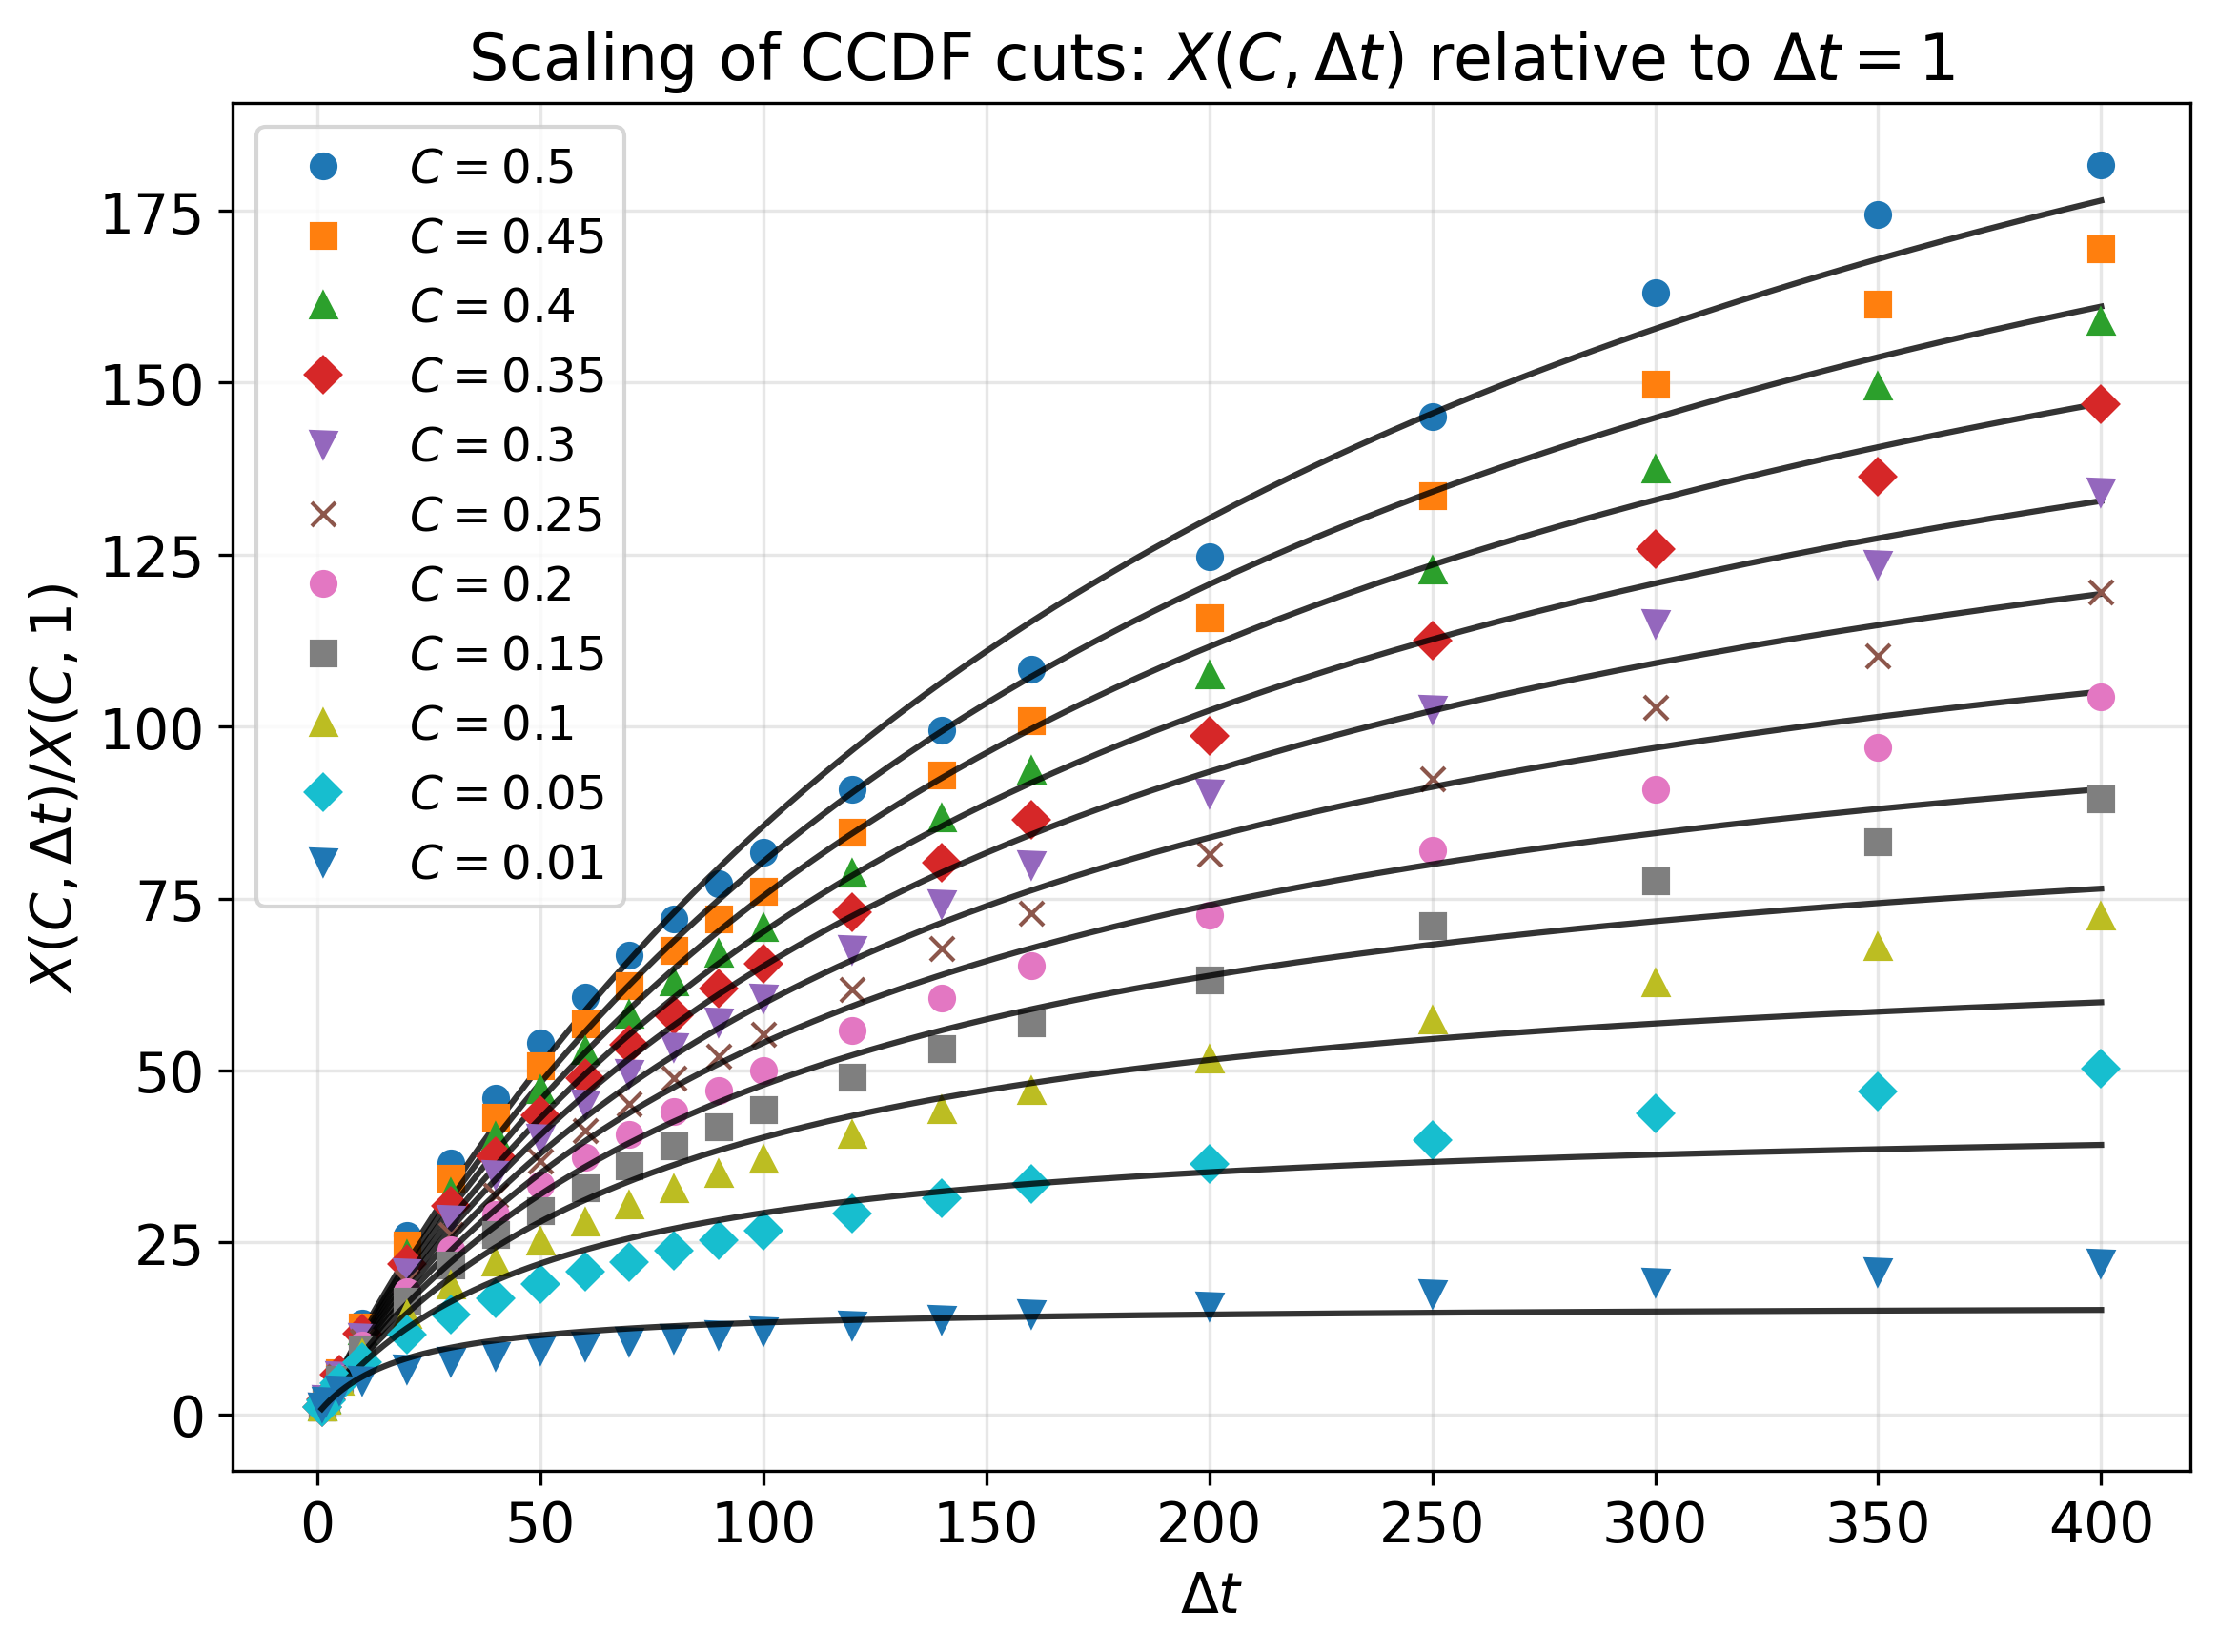
\includegraphics[width=\textwidth]{figures/ccdf_cut_scaling_investigation.png}
        \label{ccdfcutinvest}
    \end{minipage}
    \hfill
    \begin{minipage}[c]{0.35\textwidth}
        \centering
        \label{tab:fit_params}
        \begin{tabular}{ccc}
            \hline
            $C$ & $c_1$ & $c_2$ \\
            \hline
            0.50 & 1.240 & 0.00455 \\
            0.45 & 1.200 & 0.00497 \\
            0.40 & 1.160 & 0.00538 \\
            0.35 & 1.110 & 0.00589 \\
            0.30 & 1.080 & 0.00653 \\
            0.25 & 1.040 & 0.00737 \\
            0.20 & 0.998 & 0.00848 \\
            0.15 & 0.962 & 0.01010 \\
            0.10 & 0.920 & 0.01290 \\
            0.05 & 0.870 & 0.01970 \\
            0.01 & 0.829 & 0.05210 \\
            \hline
        \end{tabular}
    \end{minipage}
    \caption{Bubble displacements do not scale according to Levy distribution (left). Fitted parameters for each CCDF cut (right).}
    \label{fig:scalinginvest}
\end{figure}

By process of trial and error to find a function which scales this way, equation \ref{eq:scalefiteq} seemed the best fit.
\begin{equation}
    f(\Delta t) = \frac{c_1 \Delta t}{1 + c_2 \Delta t}
    \label{eq:scalefiteq}
\end{equation}

Equation \ref{eq:scalefiteq} uses two free parameters, $c_1$ and $c_2$, and the fit uses a least square method to obtain the corresponding $c_1$ and $c_2$ for the best fit. Each free parameter value is stored alongside the cut C that these values are associate with. Plotting $c_1$ against C gives a linear relation and $c_2$ versus C gives a decay power law which was estimated using a non-linear least squares fit as shown in figure \ref{c1c2invest}.\\

\begin{figure}[H]
    \centering
    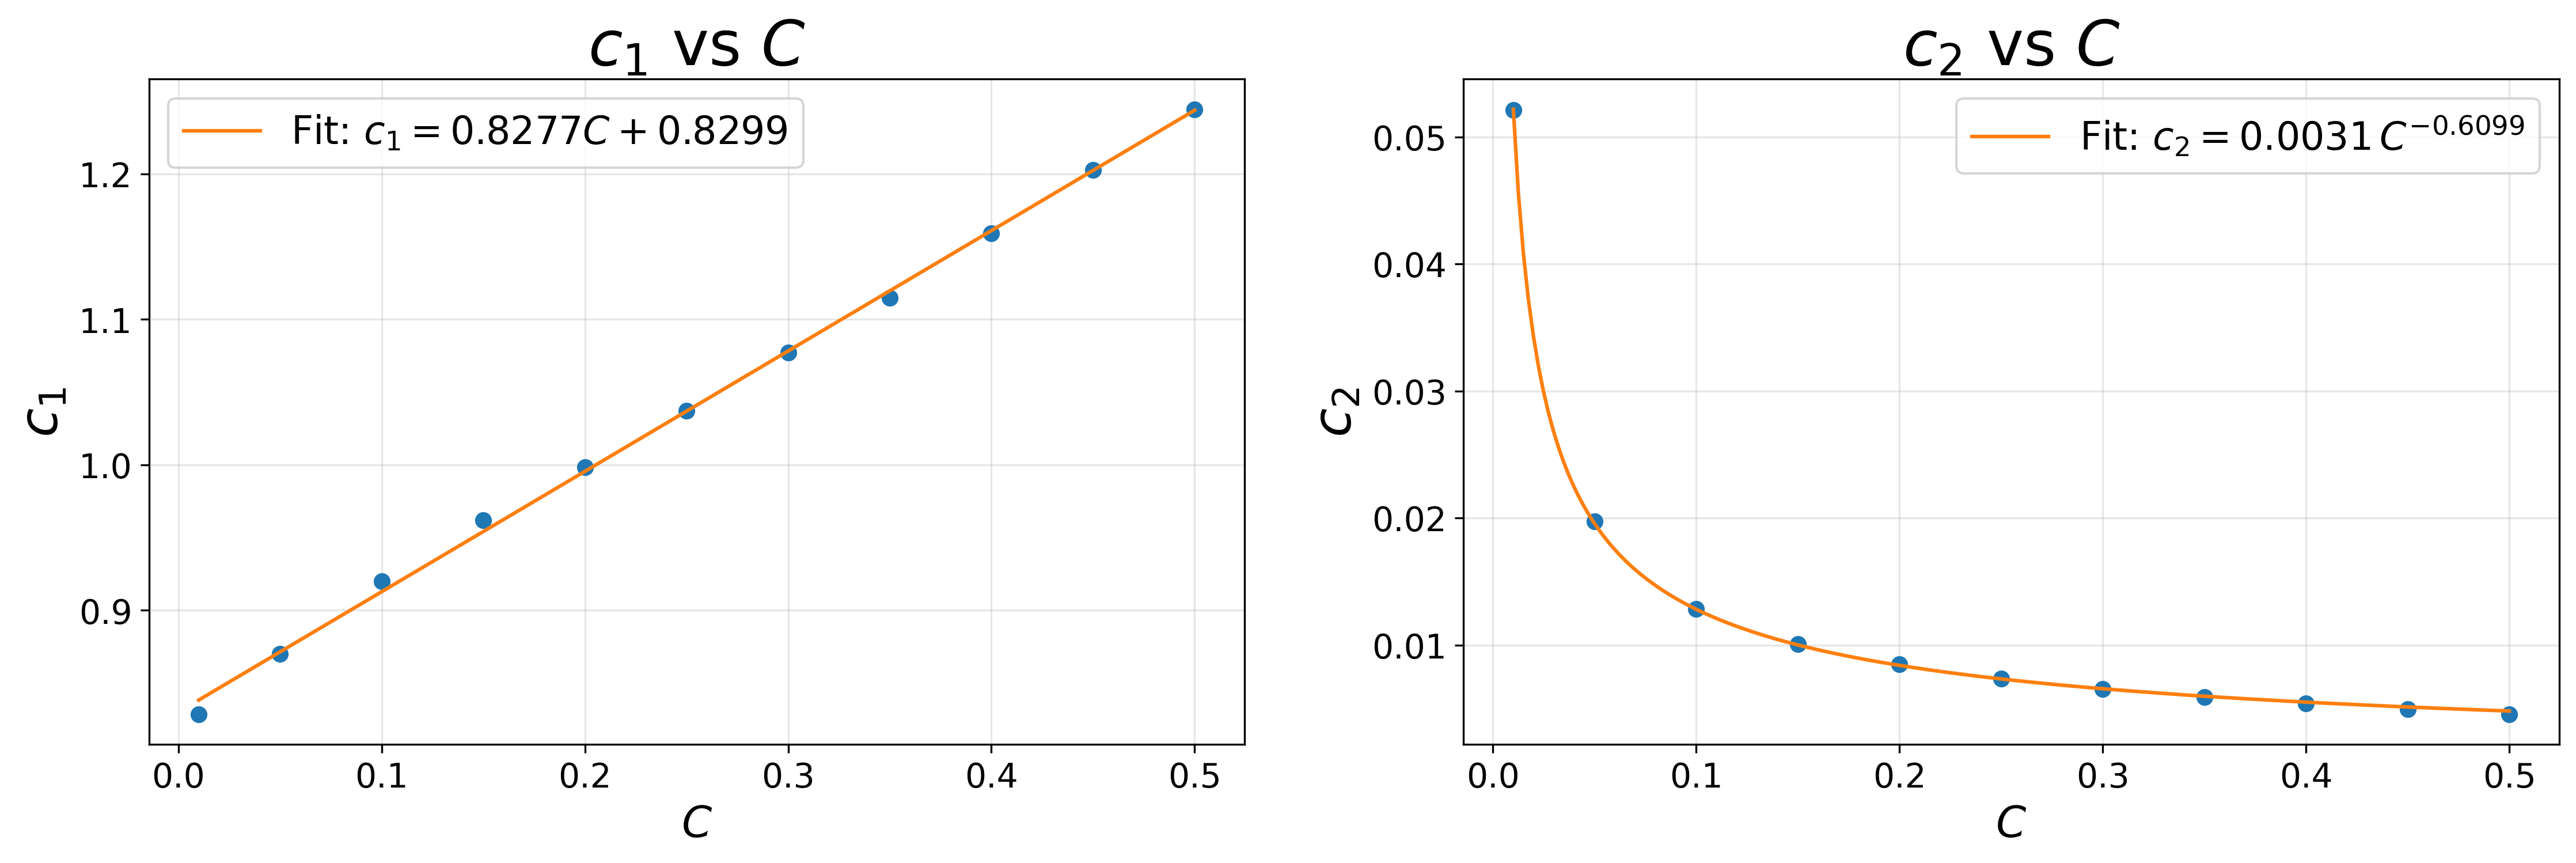
\includegraphics[width=\textwidth]{figures/c1_and_1_c2_vs_C_investigation.png}
    \caption{Linear relation for scaling of $c_1$ with respect to C, and power law fit of $c_2$ vs C}
    \label{c1c2invest}
\end{figure}

Using the plots and best fits in figure \ref{c1c2invest}, a closed form for $c_1$ and $c_2$ has been approximated:

\begin{align}
    c_1 &= 0.83(C+1) \\
    c_2 &= 0.0031\, C^{-0.61}
\end{align}

\textcolor{red}{given more time I am hoping to somehow use this slope and $C=0$ value to scale the displacement distribution PDFs onto one masterplot.}

\textcolor{red}{Peak scaling method, appendix maybe}

\subsubsection{Autocorrelation Functions}\label{subsec: Autocorrelation}
\begin{figure}[H]
    \centering
    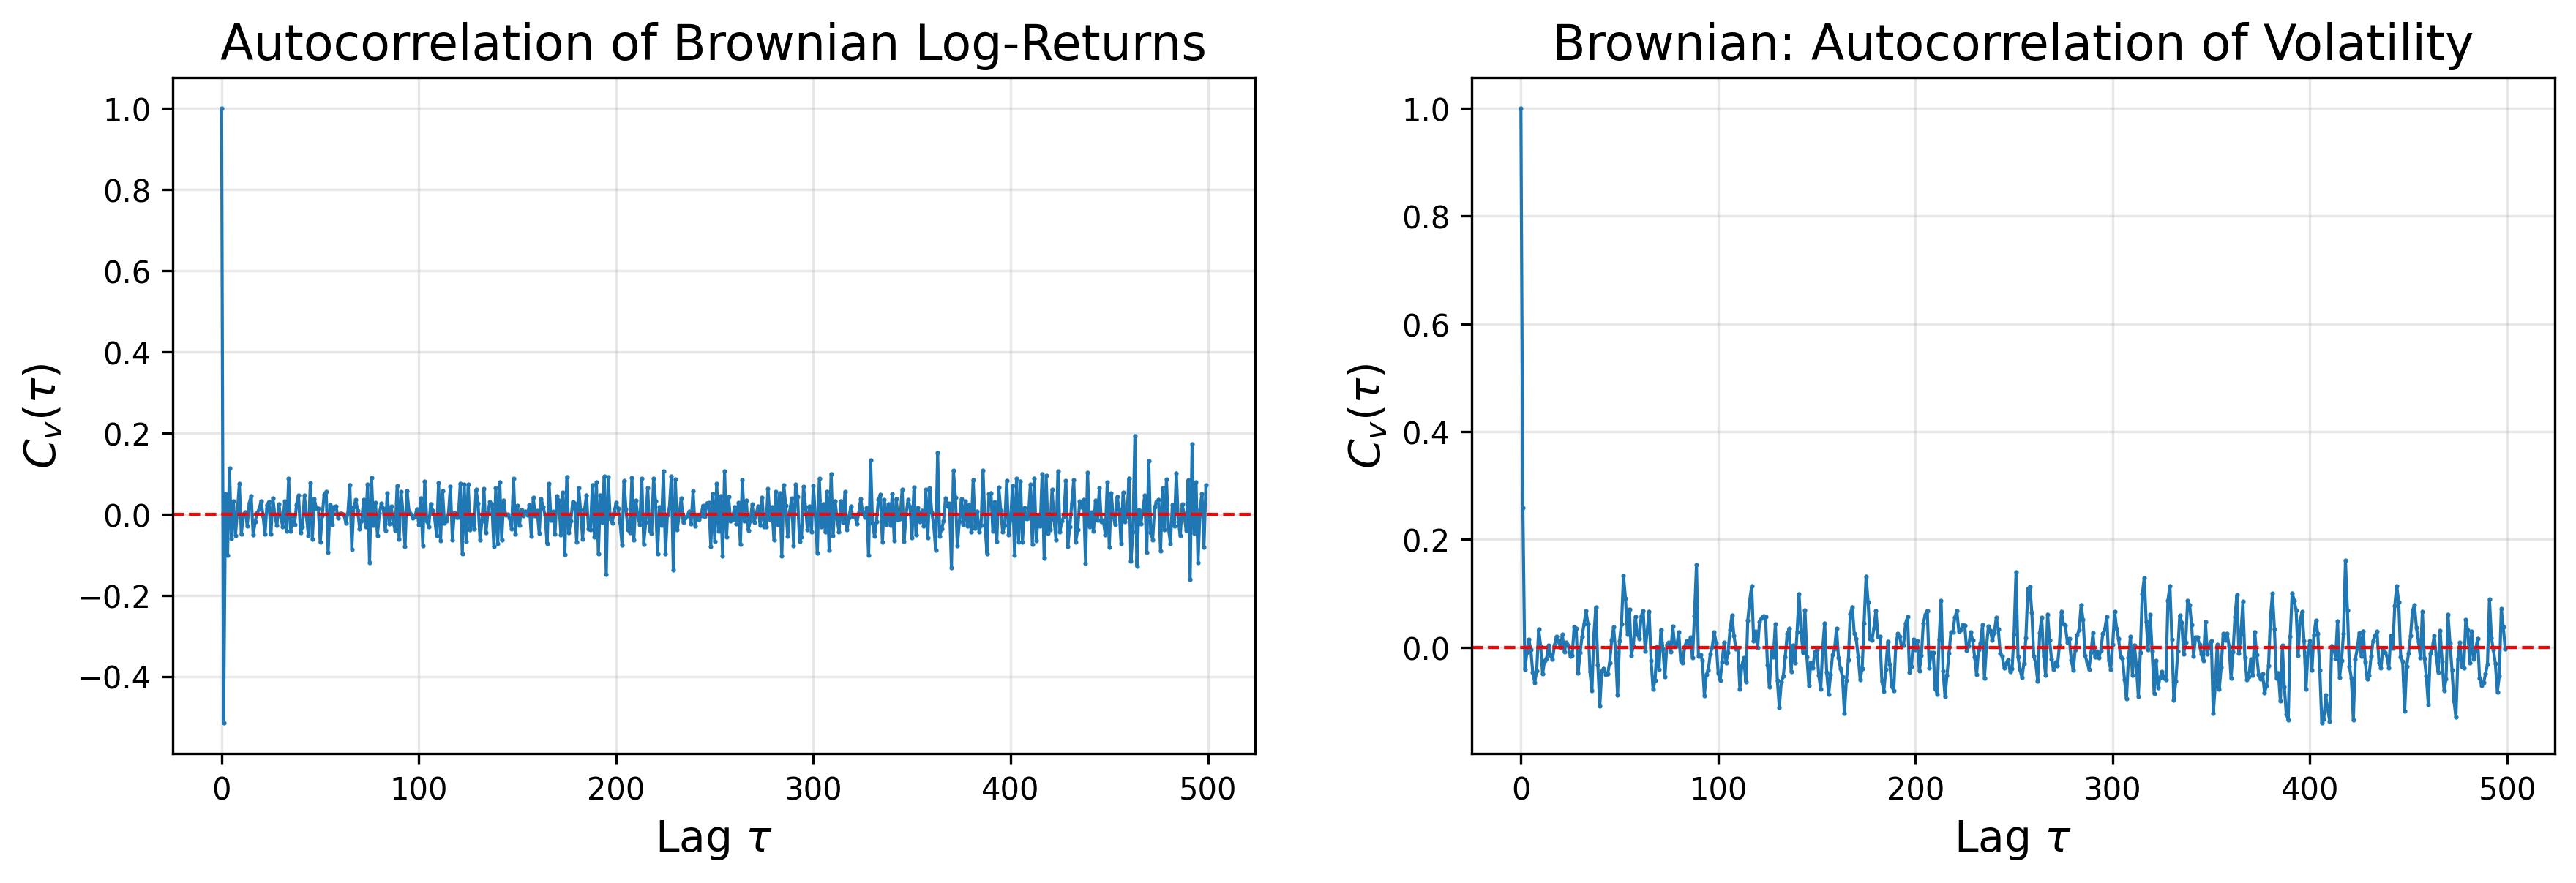
\includegraphics[width=\textwidth]{figures/lr_volatility_acf_Brownian_1x2.png}
    \caption{There is no correlation in Brownian motion, log returns or volatility in this case, as it is the baseline example of pure randomness}
    \label{fig:brownacf}
\end{figure}
As expected, the Brownian log return and volatility autocorrlation functions drop straight to zero and fluctuate there for the rest of the simulation.\\

\begin{figure}[h]
    \centering
    \begin{minipage}{0.45\textwidth}
        Figure \ref{fig:dispacf} shows the autocorrelation function for the displacement of the bubbles, as expected there is no correlation. More interestingly, the autocorrelation function for the log returns is always positive, as seen in figure \ref{fig:lrvolacf} (left). It is hard to conclude the exact physical intuition behind this but it is a key finding in this investigation nonetheless as it is unexpected that it is correlated like this.
    \end{minipage}
    \hfill
    \begin{minipage}{0.5\textwidth}
        \centering
        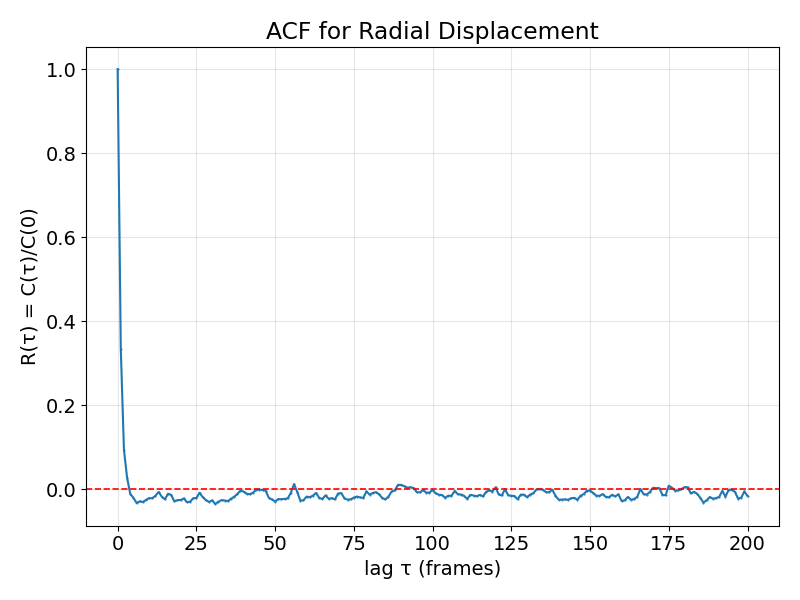
\includegraphics[width=\textwidth]{figures/dispacf.png}
        \caption{Bubble displacements remain relatively uncorrelated, ever so slightly negatively correlated}
        \label{fig:dispacf}
    \end{minipage}
\end{figure}

Figure \ref{fig:lrvolacf} (right) shows the autocorrelation of the volatility. The trend follows a power law of $\tau^{-0.4}$ and quickly drops to zero towards the end. This can be related back to figure \ref{fig:DJIA_autocorr}. The volatility autocorrelation function seems to follow a similar sort of trend, however where the DJIA differs is that the daily returns fluctuate around zero whereas the log return autocorrelation function is always slightly positive.

\begin{figure}[h!]
    \centering
    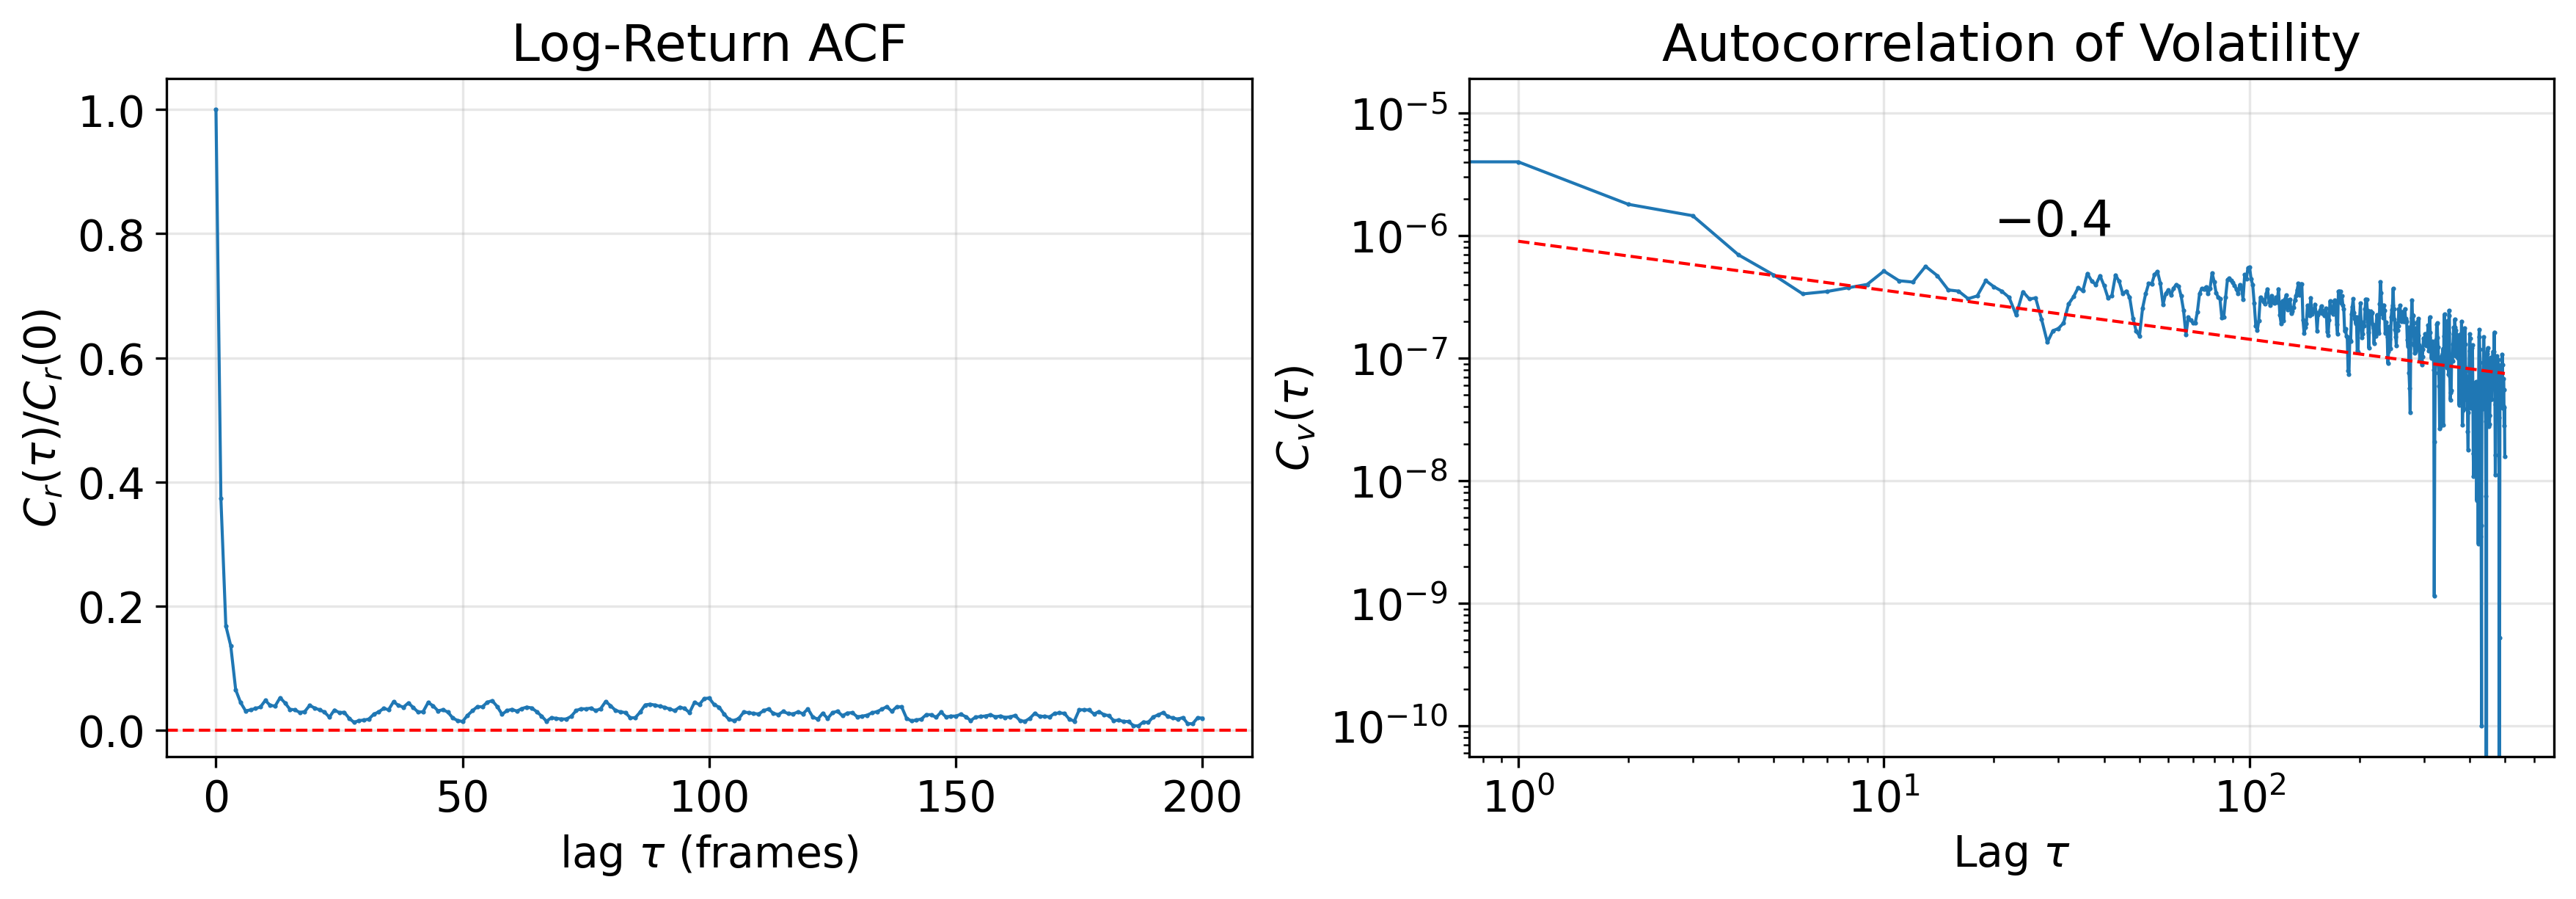
\includegraphics[width=\textwidth]{figures/lr_volatility_acf_1x2.png}
    \caption{Log return ACF unexpectedly stays ever so slightly positive, the volatility ACF follows a power law trend that can be linked back to the DJIA figure \ref{fig:DJIA_autocorr}.}
    \label{fig:lrvolacf}
\end{figure}